% !TEX root = ../main.tex

% ==========================================
% TEMA 4: DIODOS
% ==========================================
\chapter{Fenómenos de transporte de carga en semiconductores}

\section{Unión PN: Comportamiento Estático y Potencial de Contacto}

Se considera una unión PN abrupta formada por la junta de un semiconductor tipo P y un semiconductor tipo N. En los extremos de la muestra se disponen contactos metálicos óhmicos para permitir la aplicación de un potencial externo y la circulación de corriente.

\begin{figure}[h!]
    \centering
    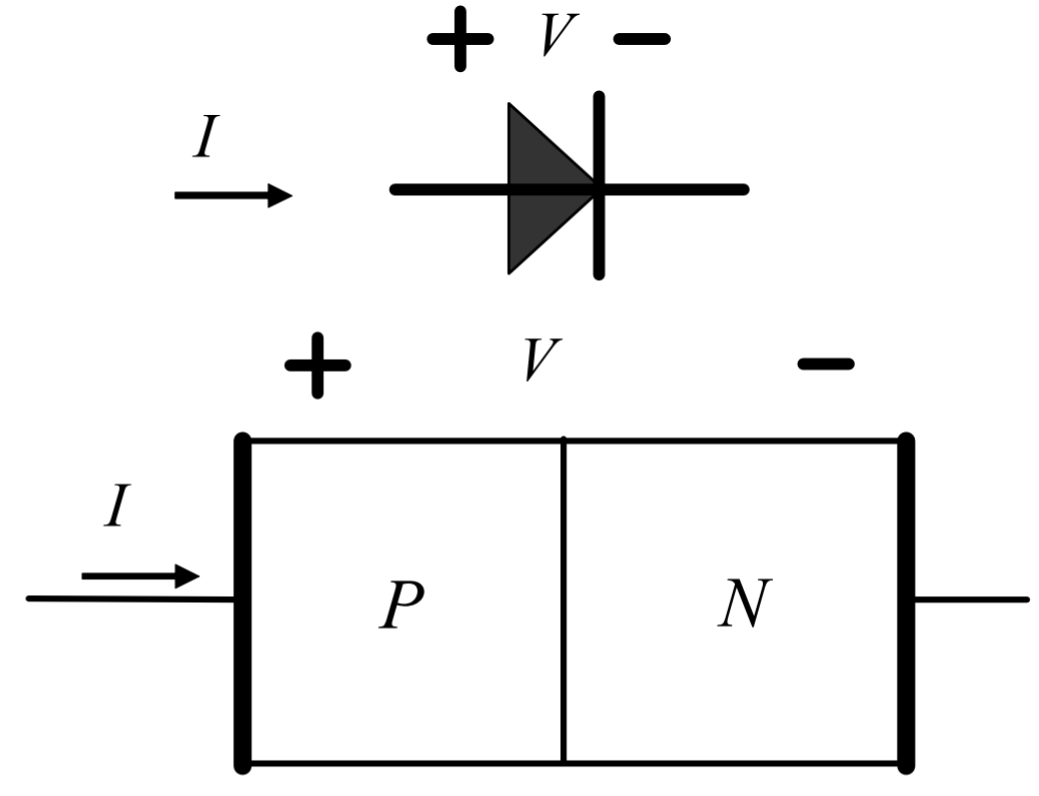
\includegraphics[width=0.35\textwidth]{imagenes/tema4/T4_1_a.png}
    \caption{Esquema físico simplificado de una unión PN con contactos metálicos.}
    \label{fig:union_pn_esquema}
\end{figure}

\newpage
\subsection{Comportamiento cualitativo y estado de equilibrio}
Al unir los materiales P y N, existe un gradiente inicial de concentración de portadores que impulsa un flujo de difusión: los huecos difunden desde el lado P hacia el lado N (a la derecha) y los electrones difunden desde el lado N hacia el lado P (a la izquierda).

\begin{figure}[h!]
    \centering
    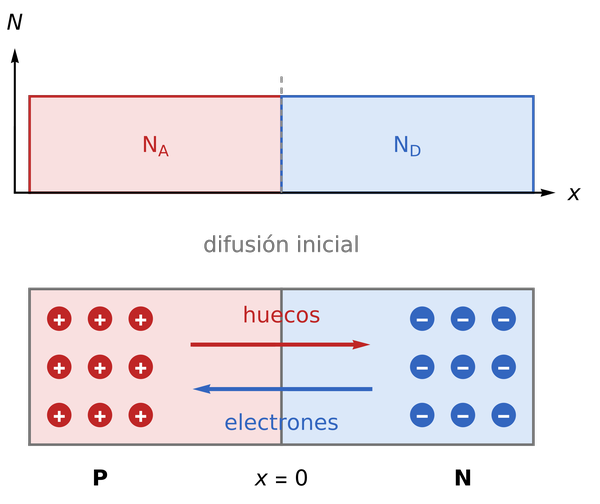
\includegraphics[width=0.5\textwidth]{imagenes/tema4/T4_1_b.png}
    \caption{Perfil de dopado ideal en una unión PN abrupta y sentido de la difusión inicial de portadores.}
    \label{fig:dopado_difusion}
\end{figure}

Al difundir los portadores libres, dejan al descubierto los iones fijos no compensados de la red cristalina: iones aceptores negativos ($N_A^-$) en el lado P e iones donadores positivos ($N_D^+$) en el lado N. Esta separación de carga genera una \textbf{Zona de Carga Espacial (ZCE)} o zona de transición cerca de la junta ($x = 0$), estableciéndose un campo eléctrico interno $\vec{E}$ dirigido del lado N al lado P.

\begin{figure}[h!]
    \centering
    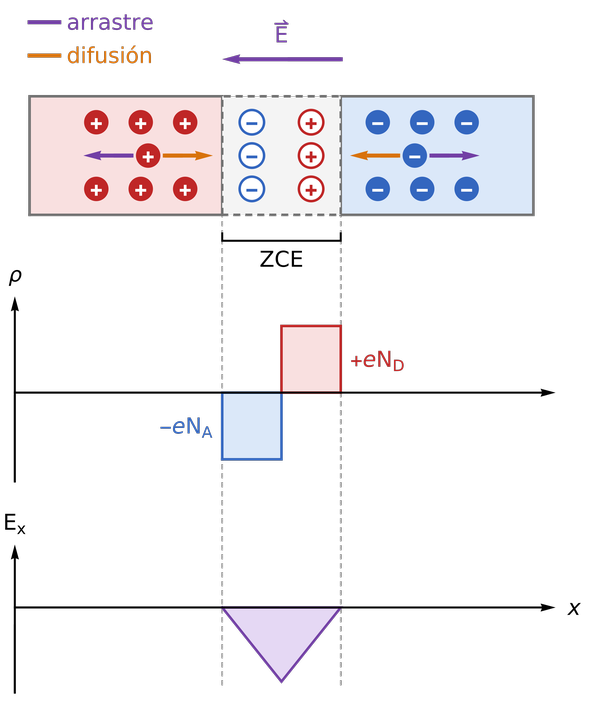
\includegraphics[width=0.5\textwidth]{imagenes/tema4/T4_1_c.png}
    \caption{Distribución de carga fija en la zona de transición, campo eléctrico interno y fuerzas de arrastre y difusión.}
    \label{fig:zce_campo_fuerzas}
\end{figure}

Este campo eléctrico ejerce una fuerza de arrastre que empuja a los electrones hacia la derecha (lado N) y a los huecos hacia la izquierda (lado P), oponiéndose al movimiento de difusión. En equilibrio térmico y sin tensión aplicada ($V_{PN} = 0$), la corriente de difusión compensa exactamente a la corriente de arrastre, resultando una intensidad nula ($I = 0$).

\begin{figure}[h!]
    \centering
    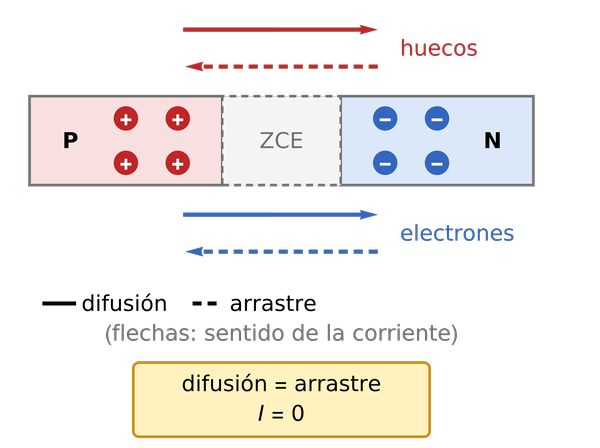
\includegraphics[width=0.5\textwidth]{imagenes/tema4/T4_1_d.png}
    \caption{Flujos de corriente por difusión y arrastre para electrones y huecos en la unión PN.}
    \label{fig:flujos_corriente}
\end{figure}

Al aplicar un potencial externo $V_{PN}$:
\begin{itemize}
    \item \textbf{Polarización directa ($V_{PN} > 0$):} Se reduce la barrera de potencial y el campo eléctrico de equilibrio. La componente de difusión predomina sobre la de arrastre, originando una corriente $I$ que crece exponencialmente con la tensión aplicada.
    \item \textbf{Polarización inversa ($V_{PN} < 0$):} Se incrementa la barrera de potencial y el campo eléctrico. La difusión queda bloqueada y solo subsiste una pequeña corriente de arrastre de portadores minoritarios, prácticamente independiente de la tensión aplicada.
\end{itemize}

\begin{figure}[h!]
    \centering
    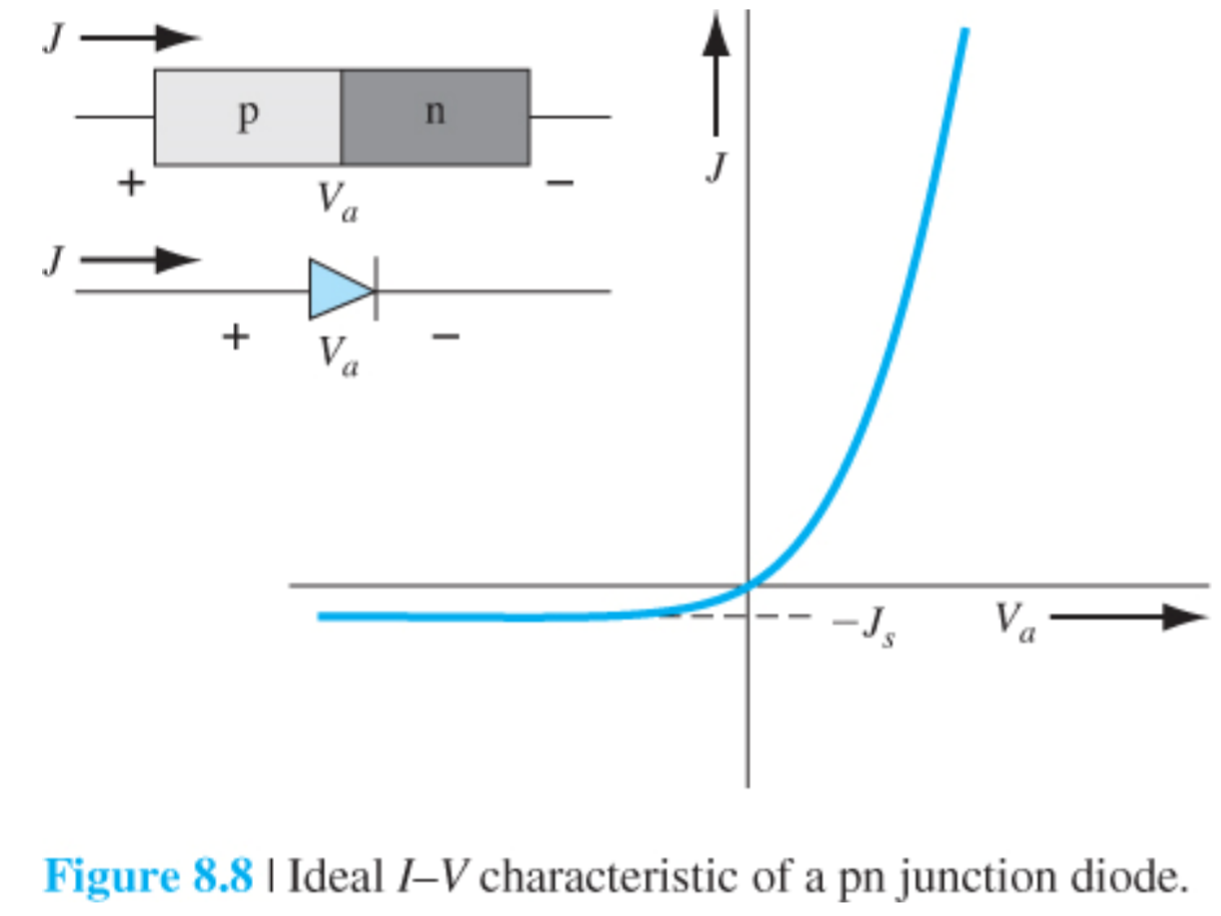
\includegraphics[width=0.65\textwidth]{imagenes/tema4/T4_1_e.png}
    \caption{Característica intensidad-voltaje ($I-V$) rectificadora ideal de una unión PN.}
    \label{fig:caracteristica_iv}
\end{figure}

\newpage
\subsection{Diagrama de bandas de energía y densidad de portadores}
Para comprender el comportamiento energético, consideremos primero los semiconductores P y N aislados. En el semiconductor tipo P, el nivel de Fermi $E_F$ se sitúa próximo a la banda de valencia $E_V$, mientras que en el tipo N se ubica cerca de la banda de conducción $E_C$.

\begin{figure}[h!]
    \centering
    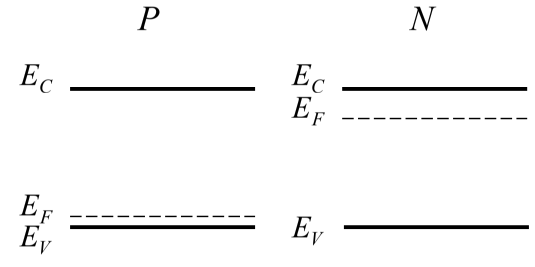
\includegraphics[width=0.65\textwidth]{imagenes/tema4/T4_1_f.png}
    \caption{Diagrama de bandas de energía para regiones P y N aisladas.}
    \label{fig:bandas_aisladas}
\end{figure}

Al formar la unión en equilibrio térmico, el nivel de Fermi $E_F$ debe permanecer constante y uniforme a lo largo de toda la muestra. Para satisfacer esta condición, las bandas de energía sufren una flexión progresiva en la zona de transición ($x_p < x < x_n$), manteniéndose constante el gap energético $E_g$.

\begin{figure}[h!]
    \centering
    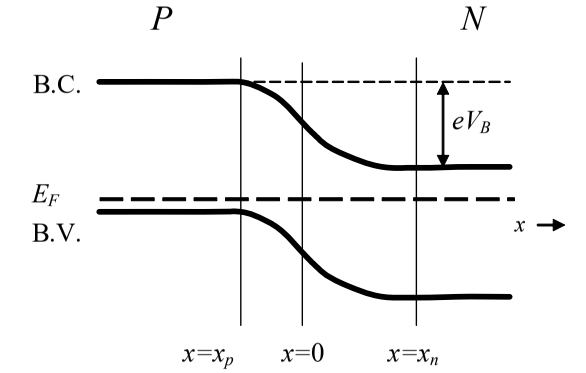
\includegraphics[width=0.5\textwidth]{imagenes/tema4/T4_1_g.png}
    \caption{Diagrama de bandas de la unión PN en equilibrio térmico con nivel de Fermi constante.}
    \label{fig:bandas_union_equilibrio}
\end{figure}

Fuera de la zona de carga espacial ($x < x_p$ y $x > x_n$), las regiones se comportan como regiones neutras idénticas a los semiconductores aislados. La curvatura suave de las bandas en la zona de transición refleja la variación espacial del potencial eléctrico $V(x)$ y la presencia del campo eléctrico $E(x) = \frac{1}{e} \frac{dE_C}{dx}$.

\newpage
Dado que la concentración de electrones depende de la separación entre la banda de conducción y el nivel de Fermi ($n = N_c \exp[(E_F - E_C)/k_B T]$), $n(x)$ aumenta exponencialmente al pasar de la región P a la N conforme $E_C(x)$ se aproxima a $E_F$. Análogamente, la densidad de huecos $p(x)$ disminuye al alejarse $E_V(x)$ del nivel de Fermi.

\begin{figure}[h!]
    \centering
    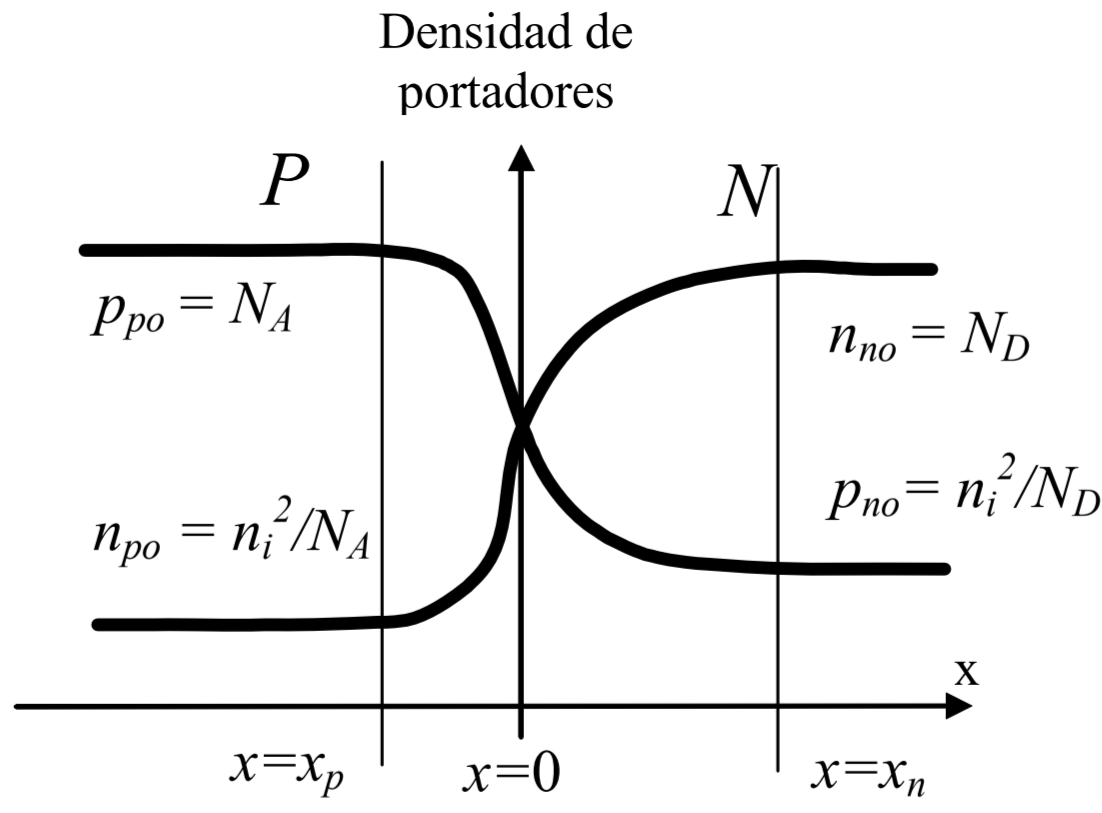
\includegraphics[width=0.5\textwidth]{imagenes/tema4/T4_1_h.png}
    \caption{Perfiles continuos de densidad de portadores $n(x)$ y $p(x)$ a lo largo de la unión PN.}
    \label{fig:densidad_portadores}
\end{figure}

\newpage
\subsection{Potencial de contacto ($V_B$)}
Imponiendo la condición de equilibrio térmico ($J_n = 0$) para la densidad de corriente de electrones:
\[
J_n = e D_n \frac{dn}{dx} + e \mu_n n E = 0 \implies -D_n \frac{dn}{dx} = n \mu_n E
\]

Aplicando la relación de Einstein ($D_n = \frac{k_B T}{e} \mu_n$), despejamos el campo eléctrico $E(x)$:
\[
E(x) = -\frac{k_B T}{e} \frac{1}{n} \frac{dn}{dx}
\]

La diferencia de potencial acumulada entre los extremos de la zona de transición ($x_p$ y $x_n$), denominada \textbf{potencial de contacto} $V_B$, se obtiene integrando el campo eléctrico:
\[
V_B = -\int_{x_p}^{x_n} E \, dx = \frac{k_B T}{e} \int_{n_{p0}}^{n_{n0}} \frac{dn}{n} = \frac{k_B T}{e} \ln\left(\frac{n_{n0}}{n_{p0}}\right)
\]

Sustituyendo las concentraciones de equilibrio $n_{n0} \approx N_D$ y $n_{p0} \approx \frac{n_i^2}{N_A}$:
\[
V_B = \frac{k_B T}{e} \ln\left(\frac{N_D N_A}{n_i^2}\right)
\]

Expresando las densidades de portadores en función de la posición del nivel de Fermi respecto al borde de la banda de conducción en cada región ($n_{n0} = N_c \exp\left[\frac{(E_F - E_C)_N}{k_B T}\right]$ y $n_{p0} = N_c \exp\left[\frac{(E_F - E_C)_P}{k_B T}\right]$):
\[
V_B = \frac{(E_F - E_C)_N - (E_F - E_C)_P}{e} > 0
\]

\newpage
\subsection{Campo eléctrico y densidad de carga espacial (Aproximación de vaciamiento total)}
Para analizar cuantitativamente el campo y el potencial en la unión, se adopta la \textbf{aproximación de vaciamiento total}, la cual asume que en la zona de transición ($x_p < x < x_n$) la densidad de portadores libres es despreciable frente a la concentración de impurezas ionizadas.

Bajo esta aproximación, la densidad de carga espacial $\rho(x)$ presenta un perfil a tramos constantes:
\[
\rho(x) = \begin{cases} -e N_A & \text{si } x_p < x < 0 \quad (\text{lado P}) \\ +e N_D & \text{si } 0 < x < x_n \quad (\text{lado N}) \end{cases}
\]

\begin{figure}[h!]
    \centering
    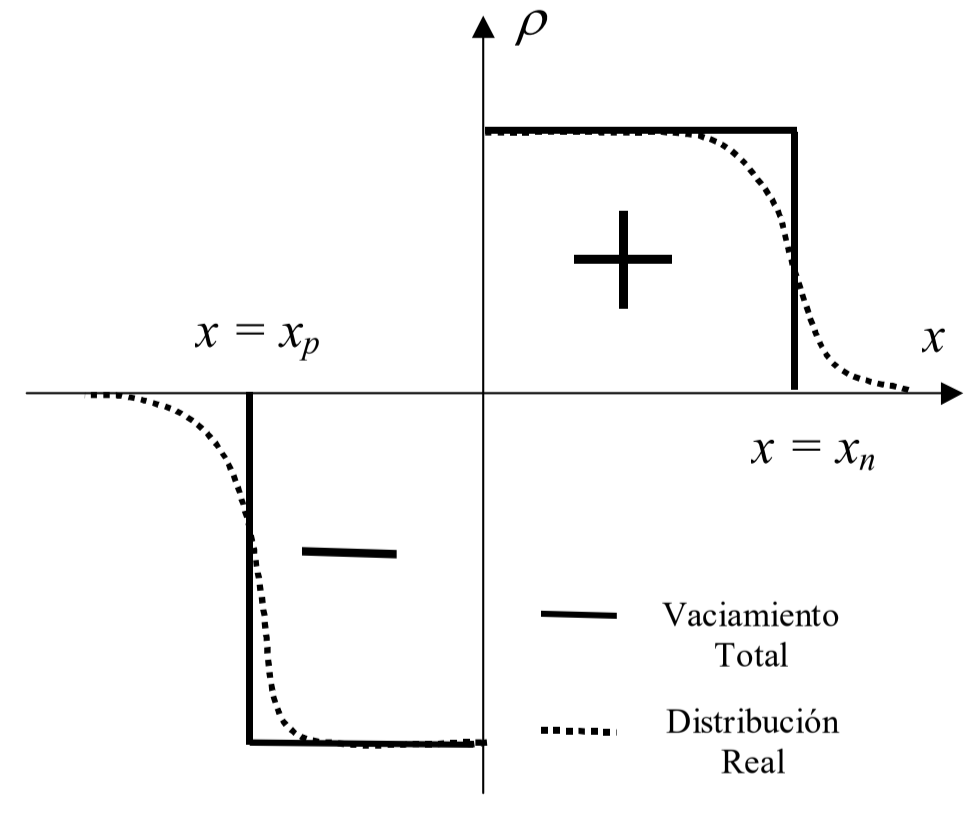
\includegraphics[width=0.5\textwidth]{imagenes/tema4/T4_1_i.png}
    \caption{Distribución de la densidad de carga espacial $\rho(x)$ bajo la aproximación de vaciamiento total frente al perfil real.}
    \label{fig:vaciamiento_total}
\end{figure}

Por la condición de neutralidad eléctrica global del dispositivo, la carga total negativa acumulada en el lado P debe ser igual en magnitud a la carga total positiva en el lado N:
\[
\int_{x_p}^{x_n} \rho(x) \, dx = 0 \implies -e N_A (-x_p) + e N_D x_n = 0 \implies N_A |x_p| = N_D x_n
\]

Geométricamente, esto implica que el área del rectángulo de carga negativa en el lado P es exactamente igual al área del rectángulo de carga positiva en el lado N.

\newpage
\subsection*{Portadores y corrientes en la unión P-N polarizada}

\subsubsection*{Cálculo de la densidad de portadores minoritarios en los bordes de la Z.C.E.}

La dinámica general de los portadores de carga en un semiconductor viene gobernada por las ecuaciones de continuidad para electrones y huecos:
\[
\frac{\partial n}{\partial t} = \mu_n \vec{\nabla} \cdot (n\vec{E}) + D_n \nabla^2 n - \frac{n - n_0}{\tau_n}
\]
\[
\frac{\partial p}{\partial t} = -\mu_p \vec{\nabla} \cdot (p\vec{E}) + D_p \nabla^2 p - \frac{p - p_0}{\tau_p}
\]

Para determinar la densidad de portadores minoritarios en los bordes de la Zona de Carga Espacial (Z.C.E.), se consideran tres hipótesis fundamentales:

\paragraph{1. Primera hipótesis: Régimen estacionario y ausencia de generación-recombinación en la Z.C.E.}
En condiciones de régimen estacionario ($\frac{\partial}{\partial t} = 0$) y suponiendo despreciable los procesos de generación y recombinación dentro de la estrecha región de carga espacial, la divergencia de las densidades de corriente se anula:
\[
\vec{\nabla} \cdot \vec{J}_p = 0 \implies \vec{\nabla} \cdot \left( \mu_p p \vec{E} - D_p \vec{\nabla} p \right) = 0
\]
Esto implica que las densidades de corriente de huecos $\vec{J}_p$ y de electrones $\vec{J}_n$ permanecen constantes a lo largo de toda la Z.C.E.

\paragraph{2. Segunda hipótesis: Débil polarización (Aproximación de quasi-equilibrio)}
Bajo condiciones de polarización débil, las corrientes netas que atraviesan la unión son cuantitativamente muy pequeñas en comparación con los elevados componentes de arrastre y difusión que se contraponen internamente en la Z.C.E. De este modo, se asume $J_p \approx 0$ y $J_n \approx 0$ localmente en la región de transición.

Considerando un modelo unidimensional donde el campo eléctrico se expresa como $E(x) = -\frac{d V_j(x)}{dx}$, la condición de corriente nula para huecos resulta:
\[
J_p = e \mu_p p E(x) - e D_p \frac{dp}{dx} \approx 0 \implies -\mu_p p \frac{d V_j(x)}{dx} \approx D_p \frac{dp}{dx}
\]

Reordenando términos y aplicando la relación de Einstein ($\frac{\mu_p}{D_p} = \frac{e}{k_B T}$):
\[
\frac{dp}{p} = -\frac{\mu_p}{D_p} d V_j(x) = -\frac{e}{k_B T} d V_j(x)
\]

Integrando desde el borde $x = x_p$ (donde el potencial de referencia es $V_j(x_p) = 0$ y la concentración de huecos es $p(x_p) = p_p$) hasta una posición genérica $x$ dentro de la Z.C.E.:
\[
\int_{p_p}^{p(x)} \frac{dp}{p} = -\frac{e}{k_B T} \int_{0}^{V_j(x)} d V_j \implies \ln\left(\frac{p(x)}{p_p}\right) = -\frac{e V_j(x)}{k_B T}
\]
\[
p(x) = p_p \exp\left(-\frac{e V_j(x)}{k_B T}\right)
\]

De manera análoga, para los electrones integrando desde la posición $x$ hasta el borde $x = x_n$ (donde $V_j(x_n) = V_B - V$ y $n(x_n) = n_n$):
\[
n(x) = n_n \exp\left(-\frac{e [V_B - V - V_j(x)]}{k_B T}\right)
\]

\paragraph{Densidades en las fronteras de la Z.C.E.}
Particularizando las expresiones obtenidas en los bordes opuestos de la zona de carga espacial:
\begin{itemize}
    \item En $x = x_n$, donde los huecos son portadores minoritarios y el potencial es $V_j(x_n) = V_B - V$:
    \[
    p(x_n) \equiv p_n = p_p \exp\left(-\frac{e (V_B - V)}{k_B T}\right)
    \]
    \item En $x = x_p$, donde los electrones son portadores minoritarios y el potencial es $V_j(x_p) = 0$:
    \[
    n(x_p) \equiv n_p = n_n \exp\left(-\frac{e (V_B - V)}{k_B T}\right)
    \]
\end{itemize}

Relacionando la barrera de potencial efectiva $V_B - V$ con los cocientes de concentraciones:
\[
V_B - V = \frac{k_B T}{e} \ln\left(\frac{p_p}{p_n}\right) = \frac{k_B T}{e} \ln\left(\frac{n_n}{n_p}\right)
\]

\paragraph{3. Tercera hipótesis: Débil nivel de inyección}
Bajo la condición de débil nivel de inyección, la variación de la concentración de portadores mayoritarios en los bordes de las zonas neutras es totalmente despreciable frente a su valor correspondiente en equilibrio térmico:
\[
p_p - p_{p0} \ll p_{p0} \implies p_p \approx p_{p0}
\]
\[
n_n - n_{n0} \ll n_{n0} \implies n_n \approx n_{n0}
\]

Dado que en equilibrio térmico ($V = 0$) se verifican las relaciones:
\[
p_{n0} = p_{p0} \exp\left(-\frac{e V_B}{k_B T}\right), \qquad n_{p0} = n_{n0} \exp\left(-\frac{e V_B}{k_B T}\right)
\]

Sustituyendo $p_p \approx p_{p0}$ y $n_n \approx n_{n0}$ en las expresiones con tensión aplicada $V$, se obtienen las \textbf{relaciones de Boltzmann} (o condiciones de contorno de Shockley):
\[
p_n = p_{n0} \exp\left(\frac{e V}{k_B T}\right), \qquad n_p = n_{p0} \exp\left(\frac{e V}{k_B T}\right)
\]

Expresando los resultados en términos del exceso de portadores minoritarios en las fronteras ($\delta p(x_n) = p_n - p_{n0}$ y $\delta n(x_p) = n_p - n_{p0}$):
\[
\delta p(x_n) = p_{n0} \left[\exp\left(\frac{e V}{k_B T}\right) - 1\right]
\]
\[
\delta n(x_p) = n_{p0} \left[\exp\left(\frac{e V}{k_B T}\right) - 1\right]
\]

\paragraph{Comportamiento físico según el régimen de polarización}
\begin{itemize}
    \item \textbf{Polarización directa ($V > 0$):} La barrera de potencial disminuye a $V_B - V$, permitiendo la difusión neta de portadores hacia las regiones opuestas. Esto provoca una \textbf{inyección exponencial de portadores minoritarios en exceso} ($p_n > p_{n0}$ y $n_p > n_{p0}$) en los bordes de la Z.C.E.
    \item \textbf{Polarización inversa ($V < 0$):} La barrera de potencial aumenta a $V_B + |V|$, inhibiendo el flujo difusivo. El campo eléctrico reforzado extrae los portadores minoritarios presentes en los bordes de la Z.C.E., produciendo un efecto de agotamiento o deplesión casi total ($p_n \approx 0$ y $n_p \approx 0$).
\end{itemize}

\newpage

\begin{figure}[h!]
    \centering
    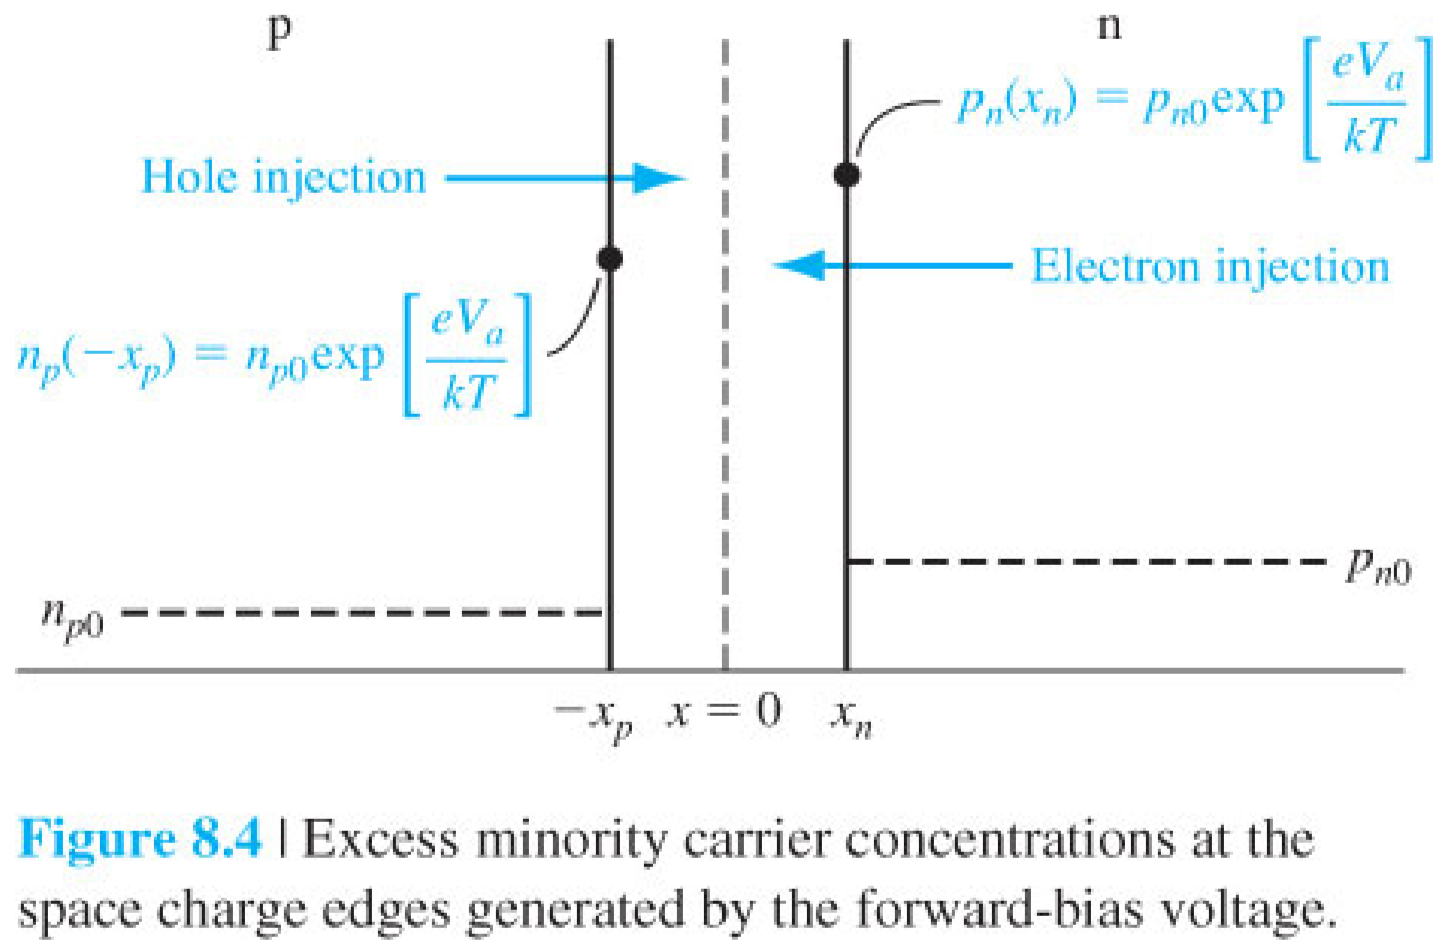
\includegraphics[width=0.60\textwidth]{imagenes/tema4/T4_1_k.png}
    \caption{Concentración de portadores minoritarios en exceso en los bordes de la zona de carga espacial bajo polarización directa.}
    \label{fig:inyeccion_boltzmann}
\end{figure}

\newpage
\begin{ejemplo}[Concentración de portadores minoritarios en los bordes de la Z.C.E.]
Calcularemos la densidad de portadores minoritarios en los bordes de la zona de carga espacial para una unión PN de silicio a $T = 300\,\text{K}$ bajo polarización directa ($V = 0,60\,\text{V}$). 

\textbf{Datos:} $N_d = 10^{16}\,\text{cm}^{-3}$, $N_a = 6 \times 10^{15}\,\text{cm}^{-3}$, $n_i = 1,5 \times 10^{10}\,\text{cm}^{-3}$, $k_B T / e \approx 0,0259\,\text{V}$.
\tcblower
En primer lugar, determinamos las concentraciones de equilibrio térmico de los portadores minoritarios en cada región:
\[
n_{p0} = \frac{n_i^2}{N_a} = \frac{(1,5 \times 10^{10}\,\text{cm}^{-3})^2}{6 \times 10^{15}\,\text{cm}^{-3}} = 3,75 \times 10^4\,\text{cm}^{-3}
\]
\[
p_{n0} = \frac{n_i^2}{N_d} = \frac{(1,5 \times 10^{10}\,\text{cm}^{-3})^2}{10^{16}\,\text{cm}^{-3}} = 2,25 \times 10^4\,\text{cm}^{-3}
\]

Aplicando las relaciones de Boltzmann con $V = 0,60\,\text{V}$:
\[
n_p(-x_p) = n_{p0} \exp\left(\frac{e V}{k_B T}\right) = (3,75 \times 10^4) \exp\left(\frac{0,60}{0,0259}\right) \approx 4,31 \times 10^{14}\,\text{cm}^{-3}
\]
\[
p_n(x_n) = p_{n0} \exp\left(\frac{e V}{k_B T}\right) = (2,25 \times 10^4) \exp\left(\frac{0,60}{0,0259}\right) \approx 2,59 \times 10^{14}\,\text{cm}^{-3}
\]

\begin{center}
    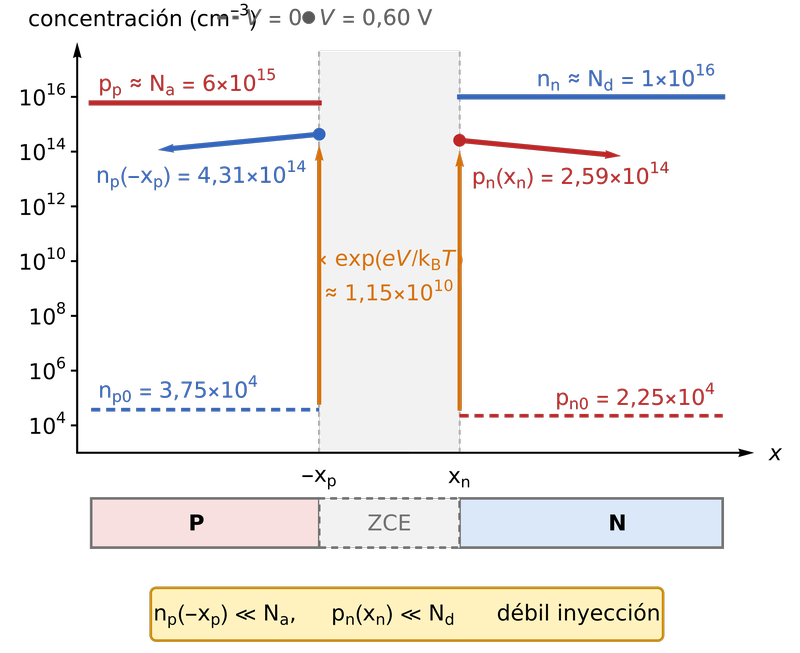
\includegraphics[width=0.6\textwidth]{imagenes/tema4/T4_E1.png}
    \captionof{figure}{.}
    \label{fig:T4_E1}
\end{center}

\textbf{Comentario físico:} 
Al aplicar una pequeña tensión en polarización directa ($0,60\,\text{V}$), las densidades de portadores minoritarios en las fronteras de la Z.C.E. aumentan en diez órdenes de magnitud. No obstante, la hipótesis de débil nivel de inyección continúa siendo plenamente válida, ya que las concentraciones inyectadas ($4,31 \times 10^{14}\,\text{cm}^{-3}$ y $2,59 \times 10^{14}\,\text{cm}^{-3}$) se mantienen sustancialmente por debajo de las densidades de portadores mayoritarios en equilibrio ($N_a = 6 \times 10^{15}\,\text{cm}^{-3}$ y $N_d = 10^{16}\,\text{cm}^{-3}$).
\end{ejemplo}

\newpage
%===========================================================
%== SUBSECCIÓN: DISTRIBUCIÓN DE PORTADORES MINORITARIOS ====
%===========================================================
\subsection*{Distribución de portadores minoritarios en las zonas neutras}

Fuera de la zona de carga espacial, en las regiones neutras P y N, el campo eléctrico es muy pequeño ($E \approx 0$). Por tanto, la dinámica de los portadores minoritarios inyectados viene gobernada exclusivamente por la difusión y la recombinación en volumen.

\paragraph{1. Huecos en el lado N ($x \ge x_n$)}
La ecuación de continuidad estacionaria para los huecos minoritarios en la región neutra N es:
\[
D_p \frac{d^2 p_n}{dx^2} - \frac{p_n - p_{n0}}{\tau_p} = 0 \implies \frac{d^2 p_n}{dx^2} = \frac{p_n - p_{n0}}{L_p^2}
\]
donde $L_p = \sqrt{D_p \tau_p}$ representa la longitud de difusión de los huecos.

La solución general de esta ecuación diferencial homogénea es:
\[
p_n(x) = p_{n0} + A e^{-(x - x_n)/L_p} + B e^{(x - x_n)/L_p}
\]

Para determinar las constantes $A$ y $B$, aplicamos las condiciones de contorno:
\begin{enumerate}[label=\alph*)]
    \item \textbf{Hipótesis de diodo largo ($x \to \infty$):} La concentración de huecos debe decrecer progresivamente hasta recuperar su valor de equilibrio térmico a medida que nos adentramos en la zona neutra:
    \[
    \lim_{x \to \infty} p_n(x) = p_{n0} \implies B = 0
    \]
    \item \textbf{Inyección en el borde de la Z.C.E. ($x = x_n$):} Por la relación de Boltzmann:
    \[
    p_n(x_n) = p_{n0} \exp\left(\frac{e V}{k_B T}\right) \implies A = p_n(x_n) - p_{n0} = p_{n0} \left[ \exp\left(\frac{e V}{k_B T}\right) - 1 \right]
    \]
\end{enumerate}

Sustituyendo los coeficientes, el perfil espacial del exceso de huecos $\delta p_n(x) = p_n(x) - p_{n0}$ resulta:
\[
p_n(x) - p_{n0} = p_{n0} \left[ \exp\left(\frac{e V}{k_B T}\right) - 1 \right] \exp\left(-\frac{x - x_n}{L_p}\right) \qquad (x \ge x_n)
\]

\paragraph{2. Electrones en el lado P ($x \le -x_p$)}
Realizando un desarrollo análogo para los electrones minoritarios en la región neutra P, la ecuación diferencial de continuidad es:
\[
\frac{d^2 n_p}{dx^2} = \frac{n_p - n_{p0}}{L_n^2} \qquad (L_n = \sqrt{D_n \tau_n})
\]

Imponiendo las condiciones de contorno de diodo largo ($\lim_{x \to -\infty} n_p(x) = n_{p0}$) y la condición de frontera de Shockley en $x = -x_p$:
\[
n_p(x) - n_{p0} = n_{p0} \left[ \exp\left(\frac{e V}{k_B T}\right) - 1 \right] \exp\left(\frac{x + x_p}{L_n}\right) \qquad (x \le -x_p)
\]

\begin{figure}[h!]
    \centering
    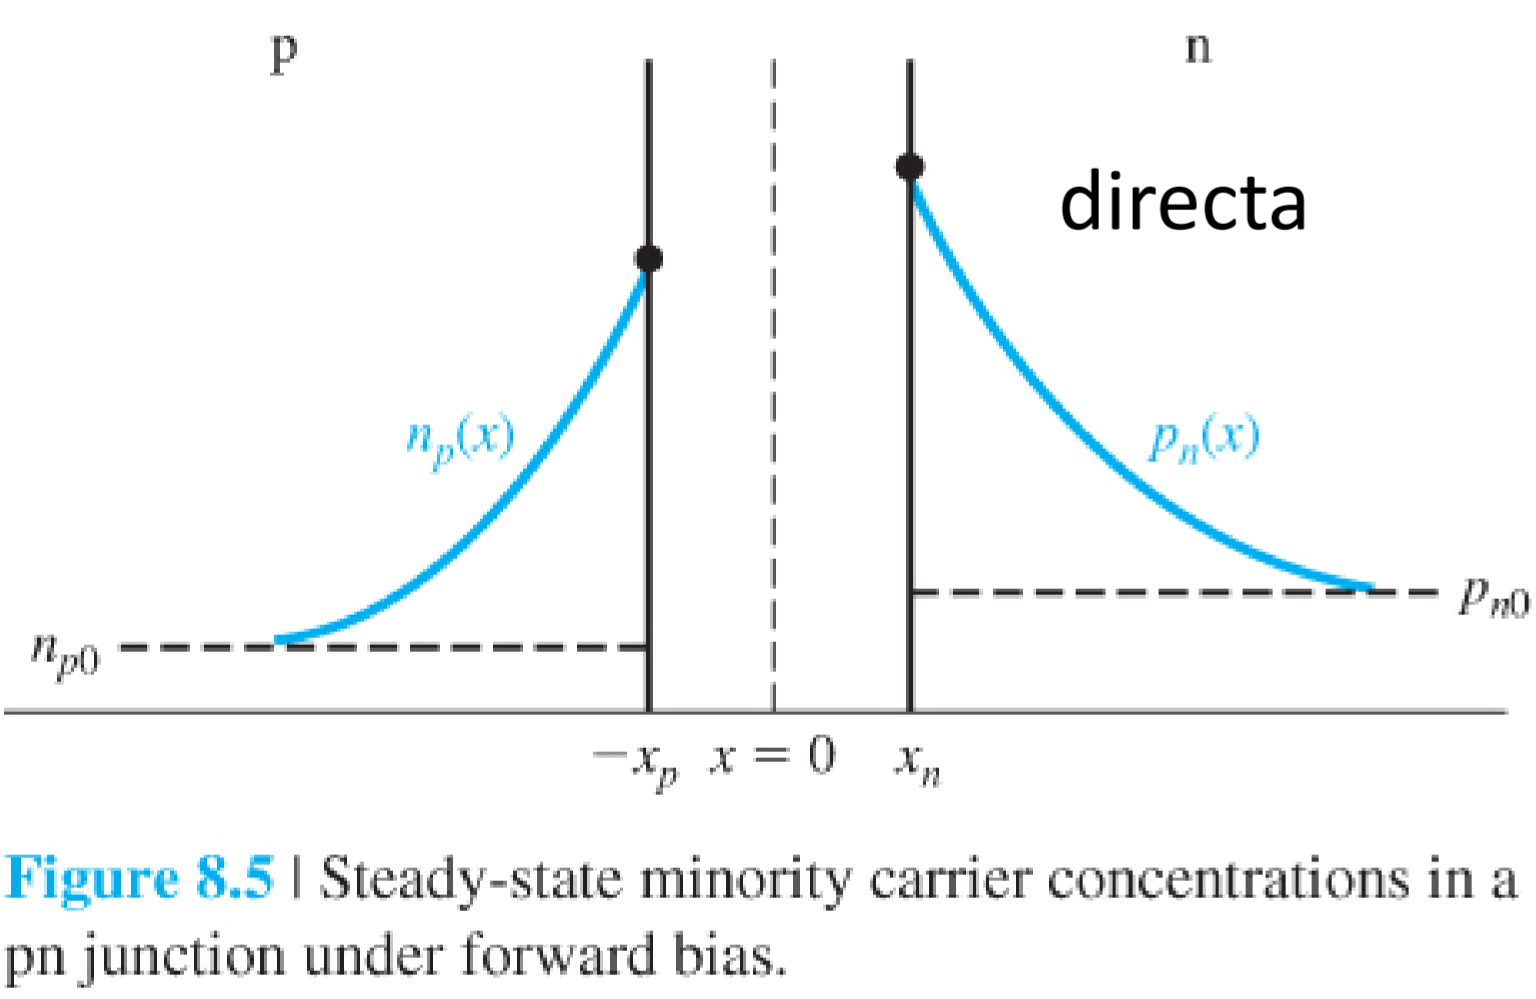
\includegraphics[width=0.60\textwidth]{imagenes/tema4/T4_1_l.png}
    \caption{Distribución estacionaria de portadores minoritarios en las regiones neutras de una unión PN bajo polarización directa.}
    \label{fig:distribucion_minoritarios_directa}
\end{figure}

\newpage
\subsubsection*{Cuasi-neutralidad en las zonas neutras}
Para preservar la neutralidad eléctrica local en las regiones neutras, la inyección de portadores minoritarios induce un ajuste equivalente en la densidad de portadores mayoritarios. Por consiguiente, el exceso espacial de mayoritarios iguala al exceso de minoritarios en cada punto:
\[
n_n(x) - n_{n0} \approx p_n(x) - p_{n0} \qquad (\text{en la región N})
\]
\[
p_p(x) - p_{p0} \approx n_p(x) - n_{p0} \qquad (\text{en la región P})
\]

\begin{figure}[h!]
    \centering
    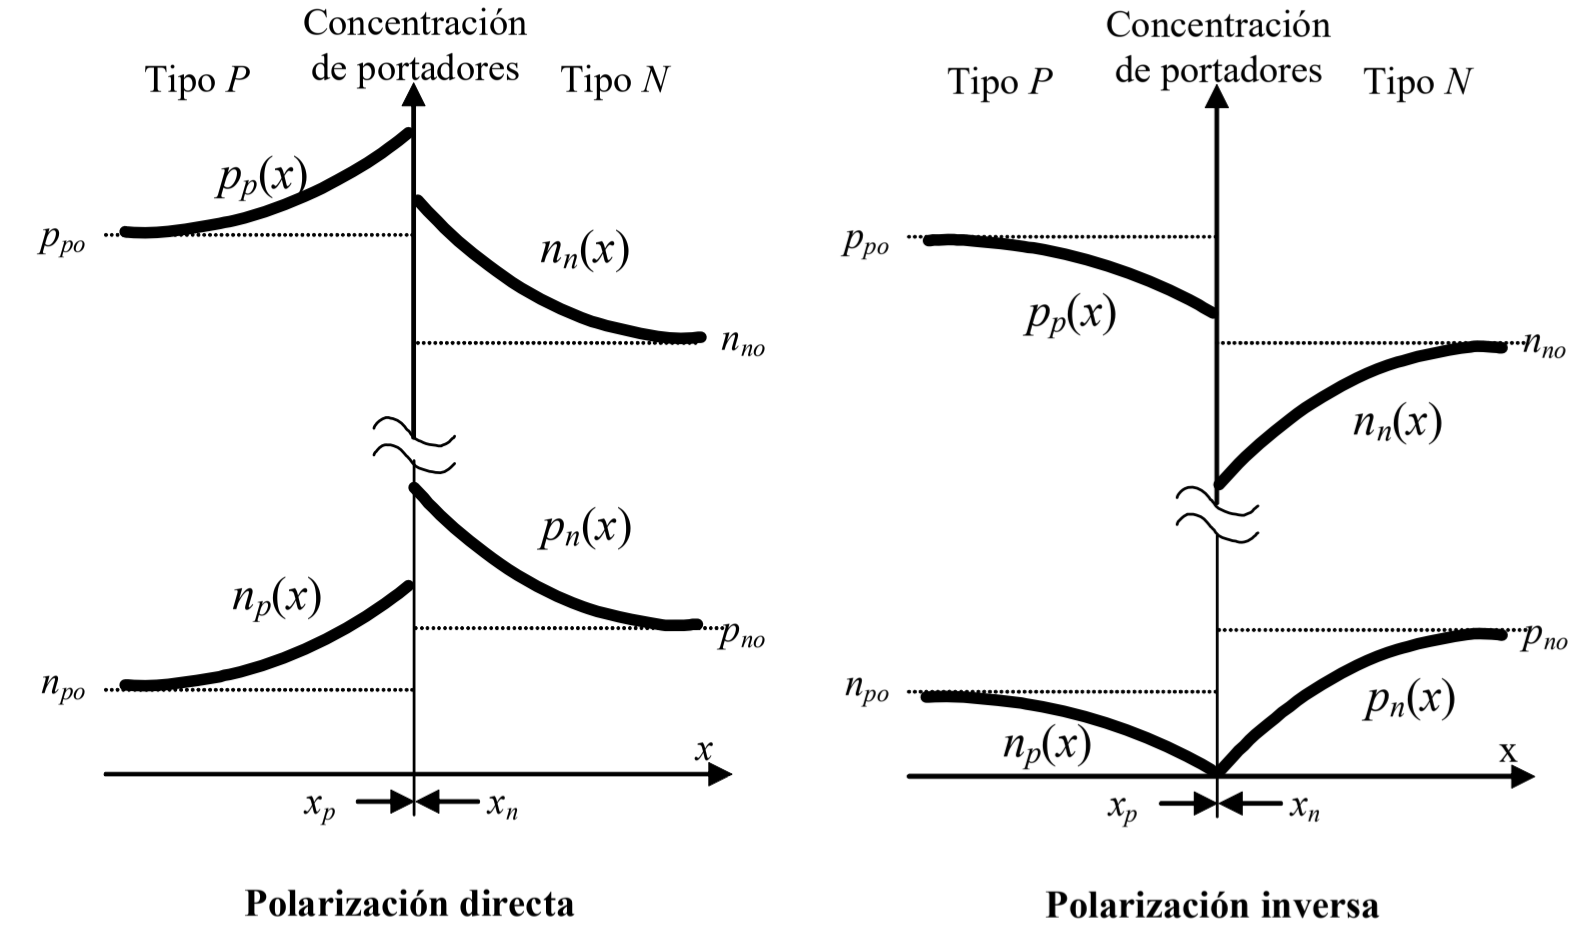
\includegraphics[width=0.75\textwidth]{imagenes/tema4/T4_1_m.png}
    \caption{Perfiles completos de densidad de portadores mayoritarios y minoritarios bajo polarización directa e inversa.}
    \label{fig:cuasi_neutralidad_perfiles}
\end{figure}

Bajo débil nivel de inyección, este pequeño exceso porcentual respecto a la elevada densidad de mayoritarios no altera sustancialmente su valor absoluto ($n_n(x) \approx N_d$ y $p_p(x) \approx N_a$), pero origina el gradiente espacial necesario para garantizar el transporte de corriente.
\newpage
%===========================================================
%== SUBSECCIÓN: CÁLCULO DE LA CORRIENTE DE LA UNIÓN PN =====
%===========================================================
\subsection*{Cálculo de la corriente de la unión P-N (Ecuación del Diodo Ideal)}

\paragraph{1. Conservación de la corriente en la Zona de Carga Espacial (Z.C.E.)}
Bajo la hipótesis de ausencia de procesos de generación y recombinación ($G = R = 0$) en el interior de la zona de carga espacial (en el intervalo $-x_p \le x \le x_n$), las densidades de corriente de electrones $J_n$ y de huecos $J_p$ permanecen estrictamente constantes a lo largo de dicha región:
\[
J_n(x) = J_n(-x_p) = J_n(x_n), \qquad J_p(x) = J_p(-x_p) = J_p(x_n) \qquad \text{para } -x_p \le x \le x_n
\]

Por la condición de continuidad, la densidad de corriente total $J$ que atraviesa el dispositivo es constante en toda la estructura:
\[
J = J_n(x) + J_p(x) = \text{constante}
\]

Evaluando la corriente total como la suma de la componente de electrones evaluada en la frontera izquierda ($x = -x_p$) y la componente de huecos evaluada en la frontera derecha ($x = x_n$):
\[
J = J_n(-x_p) + J_p(x_n)
\]

\begin{figure}[h!]
    \centering
    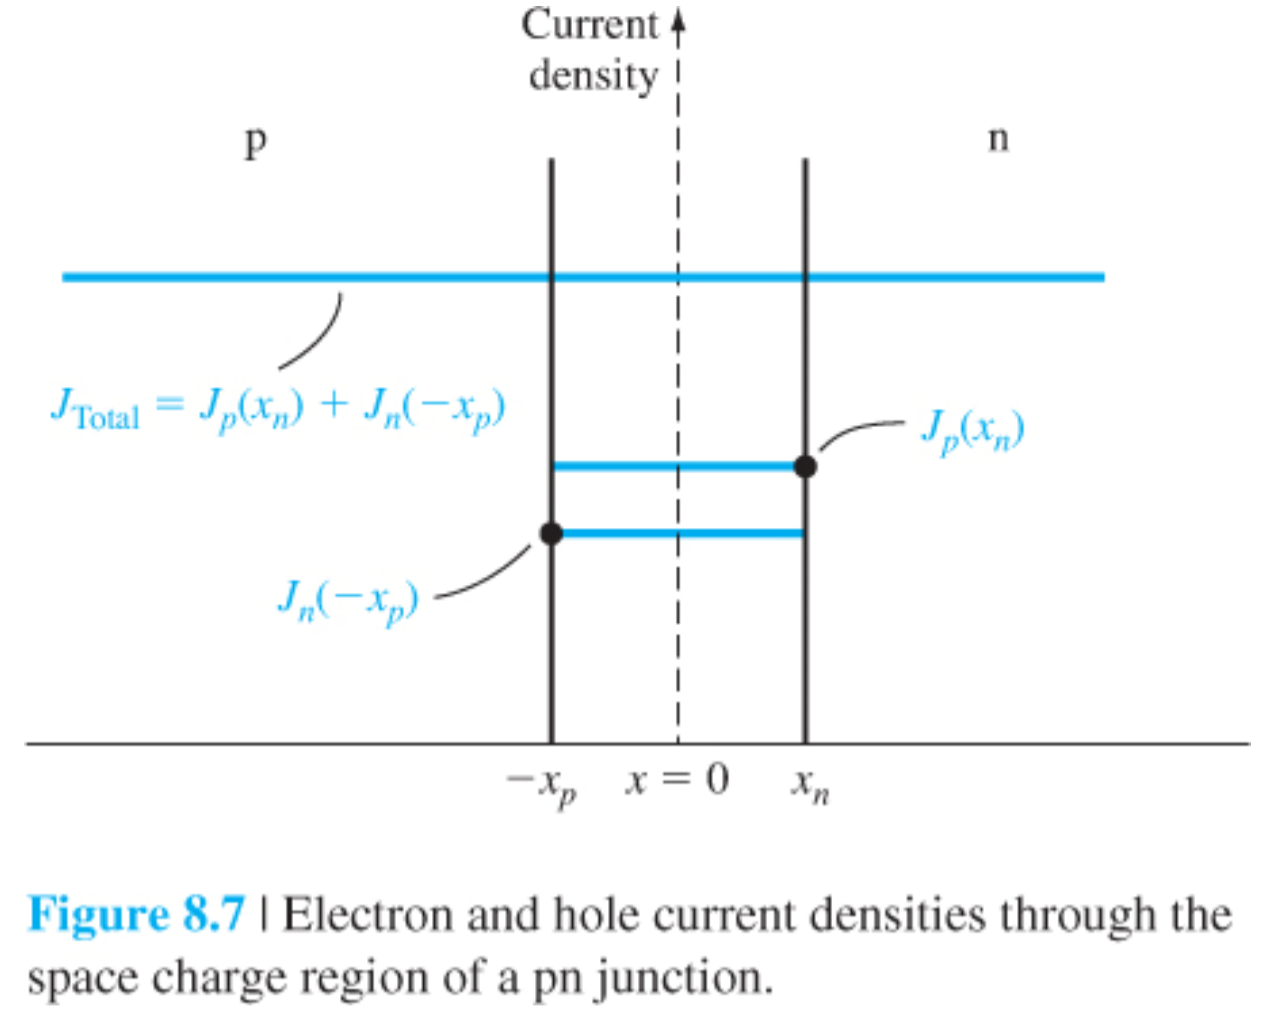
\includegraphics[width=0.60\textwidth]{imagenes/tema4/T4_1_n.png}
    \caption{Distribución de las densidades de corriente de electrones y huecos a través de la zona de carga espacial y regiones neutras.}
    \label{fig:corrientes_zce}
\end{figure}

\paragraph{2. Componentes de corriente de difusión en las zonas neutras}
En las regiones neutras fuera de la Z.C.E., el campo eléctrico es muy pequeño ($E \approx 0$). Dado que la concentración de portadores minoritarios es baja, la corriente por arrastre $e \mu n E$ resulta totalmente despreciable frente a la corriente de difusión. Por consiguiente, el transporte de portadores minoritarios se produce exclusivamente por difusión.

\begin{itemize}
    \item \textbf{Corriente de electrones en el lado P ($x \le -x_p$):}
    A partir de la distribución del exceso de electrones $n_p(x) - n_{p0} = n_{p0} \left[ \exp\left(\frac{e V}{k_B T}\right) - 1 \right] \exp\left(\frac{x + x_p}{L_n}\right)$:
    \[
    J_n(x) = e D_n \frac{d n_p(x)}{dx} = \frac{e D_n n_{p0}}{L_n} \left[ \exp\left(\frac{e V}{k_B T}\right) - 1 \right] \exp\left(\frac{x + x_p}{L_n}\right)
    \]
    Evaluando en la frontera de la Z.C.E. ($x = -x_p$):
    \[
    J_n(-x_p) = \frac{e D_n n_{p0}}{L_n} \left[ \exp\left(\frac{e V}{k_B T}\right) - 1 \right]
    \]

    \item \textbf{Corriente de huecos en el lado N ($x \ge x_n$):}
    A partir de la distribución del exceso de huecos $p_n(x) - p_{n0} = p_{n0} \left[ \exp\left(\frac{e V}{k_B T}\right) - 1 \right] \exp\left(-\frac{x - x_n}{L_p}\right)$:
    \[
    J_p(x) = -e D_p \frac{d p_n(x)}{dx} = \frac{e D_p p_{n0}}{L_p} \left[ \exp\left(\frac{e V}{k_B T}\right) - 1 \right] \exp\left(-\frac{x - x_n}{L_p}\right)
    \]
    Evaluando en la frontera de la Z.C.E. ($x = x_n$):
    \[
    J_p(x_n) = \frac{e D_p p_{n0}}{L_p} \left[ \exp\left(\frac{e V}{k_B T}\right) - 1 \right]
    \]
\end{itemize}

\paragraph{3. Ecuación ideal del diodo de Shockley}
Sumando ambas contribuciones de difusión en los bordes de la Z.C.E., obtenemos la densidad de corriente total $J$:
\[
J = e \left( \frac{D_n n_{p0}}{L_n} + \frac{D_p p_{n0}}{L_p} \right) \left[ \exp\left(\frac{e V}{k_B T}\right) - 1 \right]
\]

Definiendo la \textbf{corriente inversa de saturación} $J_0$:
\[
J_0 = e \left( \frac{D_n n_{p0}}{L_n} + \frac{D_p p_{n0}}{L_p} \right) = J_{n0} + J_{p0}
\]
donde $J_{n0} = \frac{e D_n n_i^2}{L_n N_a}$ representa la componente de corriente saturada de electrones y $J_{p0} = \frac{e D_p n_i^2}{L_p N_d}$ la componente de huecos.

Sustituyendo $J_0$, se obtiene la ecuación característica del diodo ideal de Shockley:
\[
J = J_0 \left[ \exp\left(\frac{e V}{k_B T}\right) - 1 \right]
\]

\begin{figure}[h!]
    \centering
    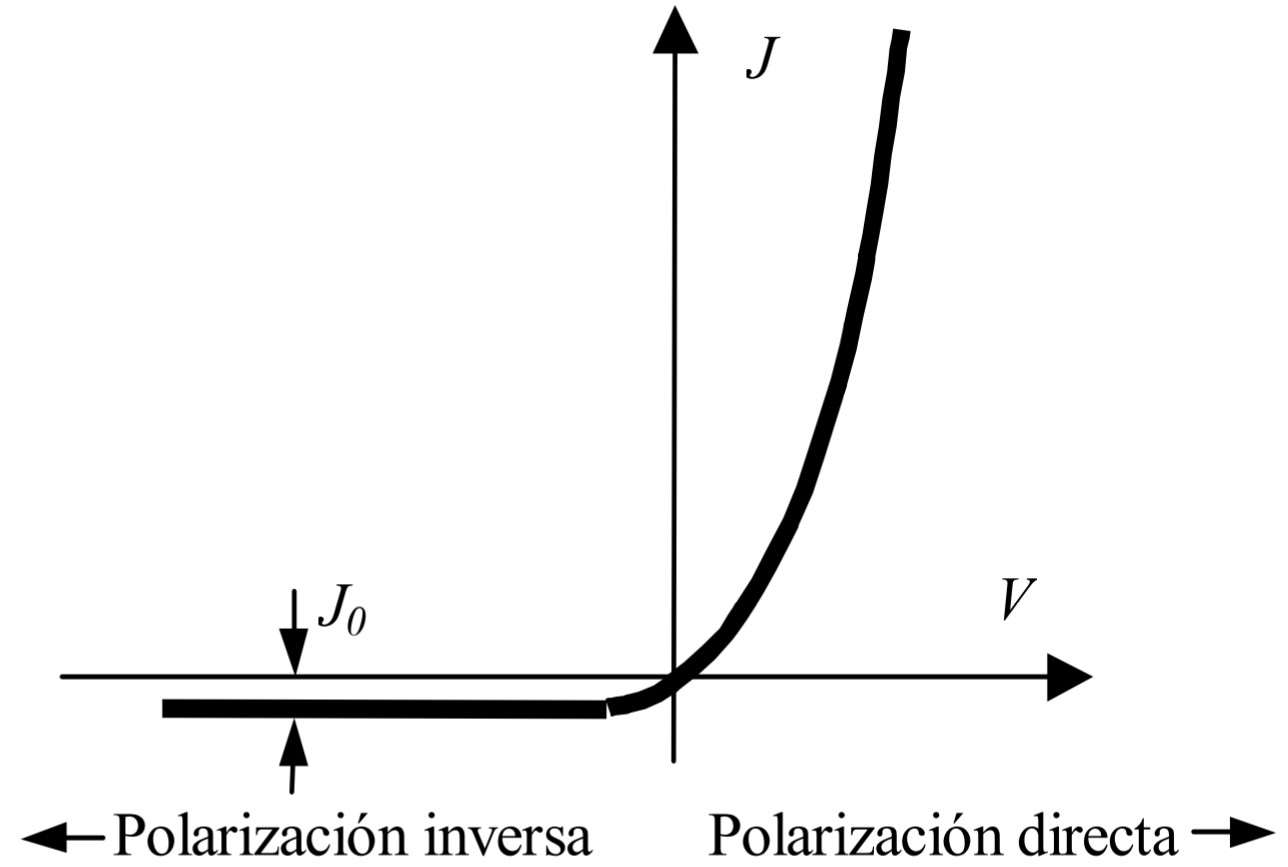
\includegraphics[width=0.55\textwidth]{imagenes/tema4/T4_1_o.png}
    \caption{Característica $J-V$ ideal de la unión PN con comportamiento rectificador en polarización directa e inversa.}
    \label{fig:caracteristica_jv_diodo}
\end{figure}

\paragraph{4. Uniones asimétricas ($P^+ N$ y $P N^+$)}
En dispositivos microelectrónicos, las uniones PN se dopan asimétricamente para seleccionar el tipo dominante de portador inyectado:

\begin{itemize}
    \item \textbf{Unión $P^+ N$ ($N_a \gg N_d$):}
    Dado que $N_a \gg N_d$, las concentraciones de minoritarios en equilibrio cumplen $n_{p0} = \frac{n_i^2}{N_a} \ll p_{n0} = \frac{n_i^2}{N_d}$.
    Consecuentemente, la corriente de saturación de huecos supera fuertemente a la de electrones ($J_{p0} \gg J_{n0}$):
    \[
    J_0 \approx J_{p0} = \frac{e D_p n_i^2}{L_p N_d} \implies J \approx J_p
    \]
    La corriente total es portada predominantemente por \textbf{huecos} inyectados desde el lado $P^+$ hacia el lado $N$.

    \item \textbf{Unión $P N^+$ ($N_d \gg N_a$):}
    Dado que $N_d \gg N_a$, las concentraciones en equilibrio cumplen $p_{n0} = \frac{n_i^2}{N_d} \ll n_{p0} = \frac{n_i^2}{N_a}$.
    Por lo tanto, $J_{n0} \gg J_{p0}$:
    \[
    J_0 \approx J_{n0} = \frac{e D_n n_i^2}{L_n N_a} \implies J \approx J_n
    \]
    La corriente total es portada fundamentalmente por \textbf{electrones} inyectados desde el lado $N^+$ hacia el lado $P$.
\end{itemize}

\newpage
\begin{ejemplo}[Densidad de corriente ideal de saturación inversa]
Determinar la densidad de corriente ideal de saturación inversa $J_s$ en una unión PN de silicio a $T = 300\,\text{K}$.

\textbf{Datos:} $N_a = N_d = 10^{16}\,\text{cm}^{-3}$, $n_i = 1,5 \times 10^{10}\,\text{cm}^{-3}$, $D_n = 25\,\text{cm}^2/\text{s}$, $D_p = 10\,\text{cm}^2/\text{s}$, $\tau_{p0} = \tau_{n0} = 5 \times 10^{-7}\,\text{s}$, $\epsilon_r = 11,7$.
\tcblower
La densidad de corriente de saturación inversa viene dada por:
\[
J_s = \frac{e D_n n_{p0}}{L_n} + \frac{e D_p p_{n0}}{L_p}
\]

Sustituyendo $n_{p0} = \frac{n_i^2}{N_a}$, $p_{n0} = \frac{n_i^2}{N_d}$, $L_n = \sqrt{D_n \tau_{n0}}$ y $L_p = \sqrt{D_p \tau_{p0}}$:
\[
J_s = e n_i^2 \left( \frac{1}{N_a} \sqrt{\frac{D_n}{\tau_{n0}}} + \frac{1}{N_d} \sqrt{\frac{D_p}{\tau_{p0}}} \right)
\]

Sustituyendo los valores numéricos:
\[
J_s = (1,6 \times 10^{-19}) \times (1,5 \times 10^{10})^2 \left( \frac{1}{10^{16}} \sqrt{\frac{25}{5 \times 10^{-7}}} + \frac{1}{10^{16}} \sqrt{\frac{10}{5 \times 10^{-7}}} \right)
\]
\[
J_s = 3,6 \times 10^{-15} \left( 7071,07 + 4472,14 \right) = 4,16 \times 10^{-11}\,\text{A/cm}^2
\]

\begin{center}
    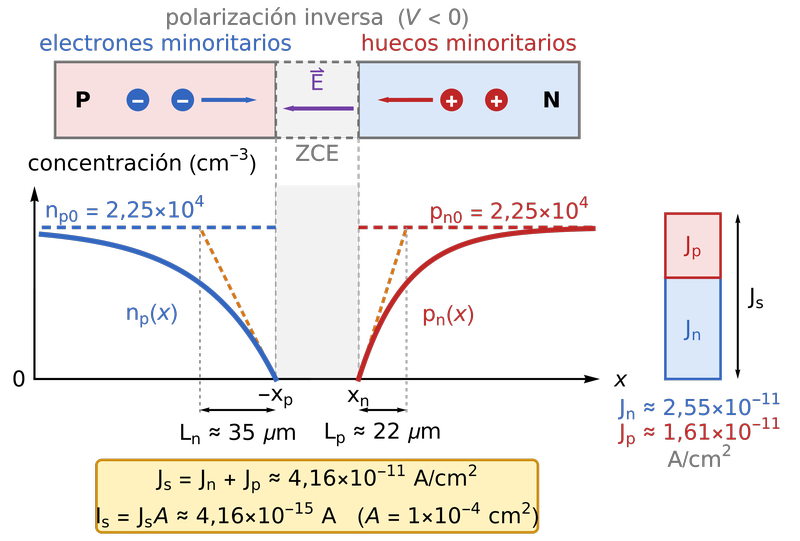
\includegraphics[width=0.6\textwidth]{imagenes/tema4/T4_E2.png}
    \captionof{figure}{.}
    \label{fig:T4_E2}
\end{center}

\textbf{Comentario físico:} 
La densidad de corriente de saturación en polarización inversa es sumamente pequeña. Para una unión PN típica con un área transversal $A = 10^{-4}\,\text{cm}^2$, la corriente inversa de saturación absoluta resulta $I_s = J_s A = 4,16 \times 10^{-15}\,\text{A}$.

Debido a esta corriente sumamente reducida, se define el \textbf{voltaje umbral} ($V_{\text{th}}$) como la tensión en directa mínima a partir de la cual se observa una conducción de corriente apreciable. Por encima del voltaje umbral, la corriente crece de forma exponencial, manteniendo la caída de tensión en la unión prácticamente constante.
\end{ejemplo}

\newpage
\begin{ejemplo}[Variación del voltaje en directa con la temperatura]
Determinar el cambio en el voltaje en directa de una unión PN de silicio para mantener constante la corriente al variar la temperatura. Inicialmente el diodo está polarizado a $V_{a1} = 0,60\,\text{V}$ a $T_1 = 300\,\text{K}$. Se supone que la temperatura se incrementa hasta $T_2 = 310\,\text{K}$ y que el gap del silicio es $E_g = 1,12\,\text{eV}$.
\tcblower
La densidad de corriente en directa depende de la temperatura según:
\[
J \propto \exp\left(-\frac{E_g}{k_B T}\right) \exp\left(\frac{e V_a}{k_B T}\right) = \exp\left(-\frac{E_g - e V_a}{k_B T}\right)
\]

Tomando el cociente entre las densidades de corriente a ambas temperaturas:
\[
\frac{J_2}{J_1} = \frac{\exp\left(-\frac{E_g - e V_{a2}}{k_B T_2}\right)}{\exp\left(-\frac{E_g - e V_{a1}}{k_B T_1}\right)}
\]

Imponiendo la condición de corriente constante ($J_1 = J_2 \implies J_2 / J_1 = 1$):
\[
\frac{E_g - e V_{a2}}{k_B T_2} = \frac{E_g - e V_{a1}}{k_B T_1} \implies \frac{1,12 - V_{a2}}{310} = \frac{1,12 - 0,60}{300}
\]

Despejando $V_{a2}$:
\[
\frac{1,12 - V_{a2}}{310} = \frac{0,52}{300} \implies 1,12 - V_{a2} = 0,5373 \implies V_{a2} = 0,5827\,\text{V}
\]

\begin{center}
    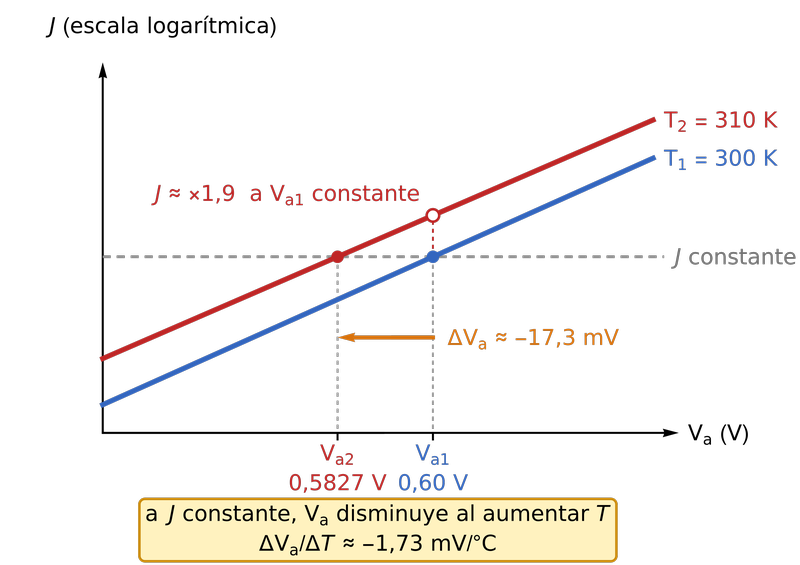
\includegraphics[width=0.6\textwidth]{imagenes/tema4/T4_E3.png}
    \captionof{figure}{.}
    \label{fig:T4_E3}
\end{center}

\textbf{Comentario físico:} 
El cambio en la tensión en directa necesaria para mantener constante la corriente es $\Delta V_a = 0,5827\,\text{V} - 0,60\,\text{V} = -0,0173\,\text{V} = -17,3\,\text{mV}$ para un incremento térmico de $10\,^\circ\text{C}$ (lo que equivale a un coeficiente de temperatura aproximado de $-1,73\,\text{mV/}^\circ\text{C}$).
\end{ejemplo}

\newpage
\subsection*{Corrientes en función de la posición}

A lo largo de toda la estructura de la unión PN, la densidad de corriente total $J_{\text{Total}}$ debe mantenerse constante por conservación de la carga en régimen estacionario. Sin embargo, la contribución relativa de las componentes de electrones $J_n(x)$ y huecos $J_p(x)$ varía espacialmente.

\begin{figure}[h!]
    \centering
    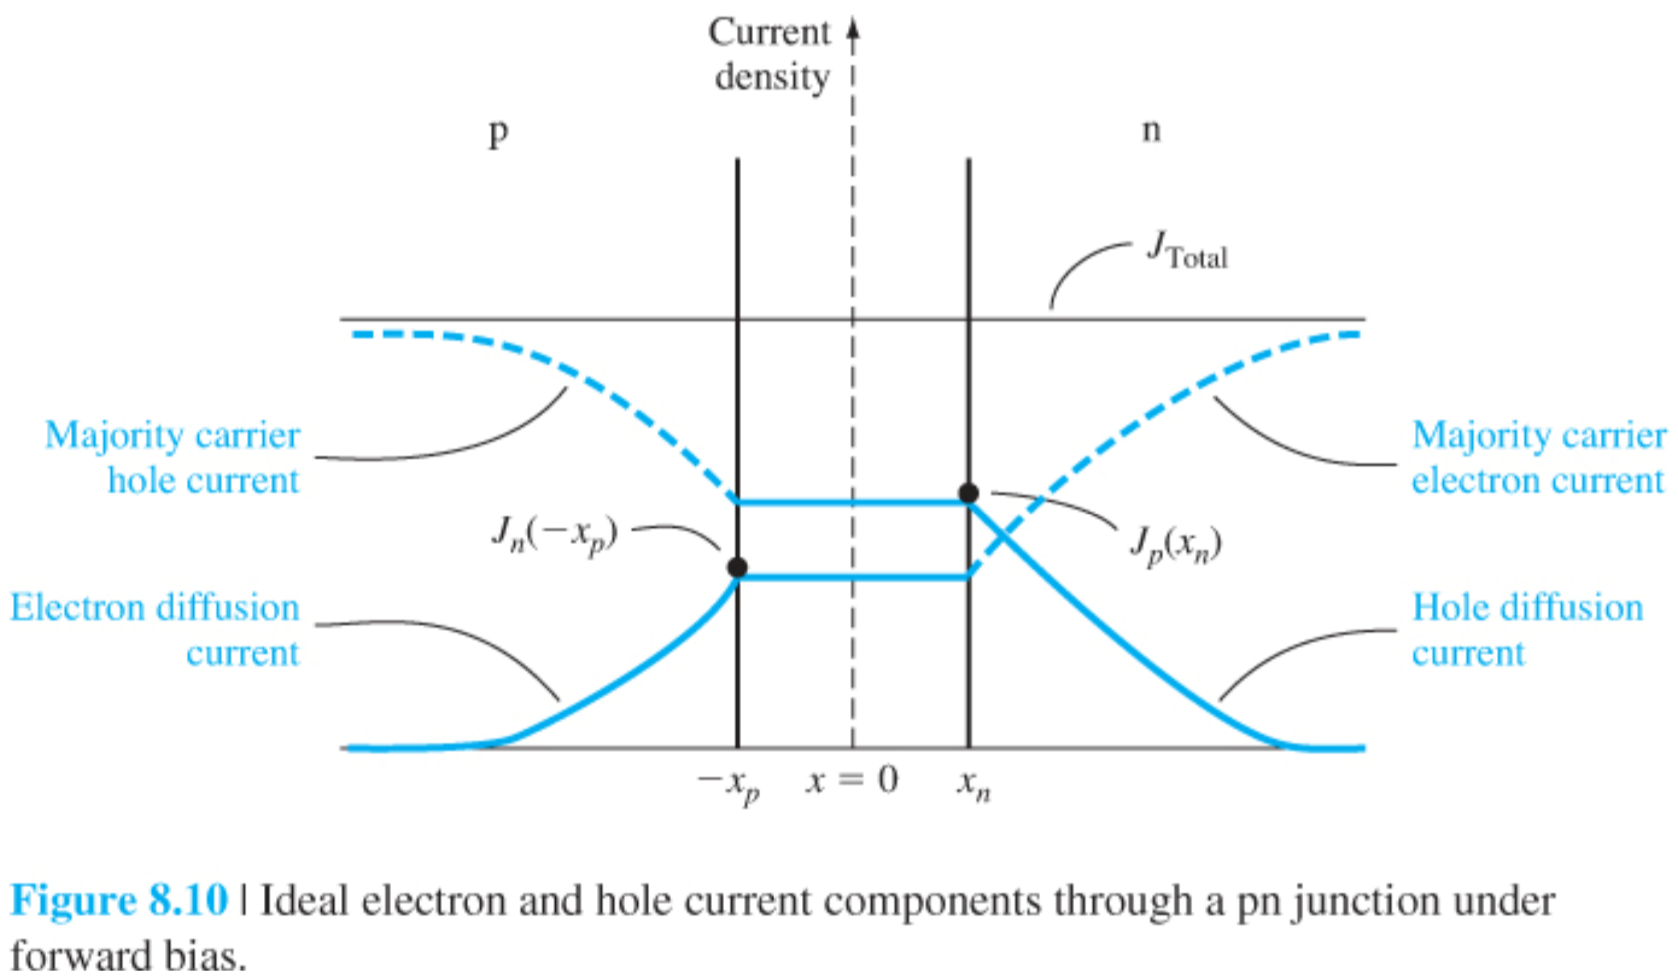
\includegraphics[width=0.65\textwidth]{imagenes/tema4/T4_1_p.png}
    \caption{Distribución espacial de las componentes de densidad de corriente de electrones y huecos en una unión PN bajo polarización directa.}
    \label{fig:corrientes_posicion}
\end{figure}

\begin{itemize}
    \item \textbf{Región P ($x \le -x_p$):}
    La corriente de electrones (minoritarios) es puramente de difusión:
    \[
    J_n(x) = e D_n \frac{d n_p(x)}{dx} = \frac{e D_n n_{p0}}{L_n} \left[ \exp\left(\frac{e V}{k_B T}\right) - 1 \right] \exp\left(\frac{x + x_p}{L_n}\right)
    \]
    La corriente de huecos (mayoritarios) se obtiene por diferencia con la corriente total:
    \[
    J_p(x) = J_{\text{Total}} - J_n(x)
    \]
    A medida que nos alejamos de la Z.C.E. hacia el contacto metálico ($x \to -\infty$), el exceso de electrones inyectados se recombina, de modo que la corriente de difusión de minoritarios tiende a cero ($J_n \to 0$) y la corriente total es transportada enteramente por arrastre de huecos mayoritarios.

    \item \textbf{Zona de Carga Espacial ($-x_p < x < x_n$):}
    Suponiendo ausencia de generación y recombinación en la Z.C.E., tanto $J_n(x)$ como $J_p(x)$ se mantienen constantes en todo el tramo:
    \[
    J_n(x) = J_n(-x_p), \qquad J_p(x) = J_p(x_n)
    \]

    \item \textbf{Región N ($x \ge x_n$):}
    La corriente de huecos (minoritarios) es de difusión:
    \[
    J_p(x) = -e D_p \frac{d p_n(x)}{dx} = \frac{e D_p p_{n0}}{L_p} \left[ \exp\left(\frac{e V}{k_B T}\right) - 1 \right] \exp\left(-\frac{x - x_n}{L_p}\right)
    \]
    La corriente de electrones (mayoritarios) compensa el resto de la corriente total:
    \[
    J_n(x) = J_{\text{Total}} - J_p(x)
    \]
    Conforme $x \to \infty$, la recombinación reduce la corriente de difusión de huecos a cero, pasando la corriente total a ser transportada de forma exclusiva por arrastre de electrones mayoritarios.
\end{itemize}

\subsection*{Cuasiniveles de Fermi}

En condiciones de desequilibrio (cuando existe polarización aplicada o fotogeneración), el nivel de Fermi único $E_F$ deja de ser válido para describir simultáneamente las concentraciones de electrones y huecos. Para extender las expresiones de equilibrio térmico, se definen dos \textbf{cuasiniveles de Fermi} independientes: $E_{FN}(x)$ para electrones en la banda de conducción y $E_{FP}(x)$ para huecos en la banda de valencia.

Las densidades locales de portadores se expresan como:
\[
n(x) = N_c \exp\left[\frac{E_{FN}(x) - E_C(x)}{k_B T}\right]
\]
\[
p(x) = N_v \exp\left[\frac{E_V(x) - E_{FP}(x)}{k_B T}\right]
\]

El producto de portadores fuera del equilibrio resulta:
\[
n(x) p(x) = n_i^2 \exp\left[\frac{E_{FN}(x) - E_{FP}(x)}{k_B T}\right]
\]

\paragraph{1. Polarización inversa ($V < 0$)}
Bajo polarización inversa, la extracción de portadores minoritarios en los bordes de la Z.C.E. produce un defecto local de concentración ($n p < n_i^2$). La separación entre cuasiniveles refleja esta disminución:

\begin{figure}[h!]
    \centering
    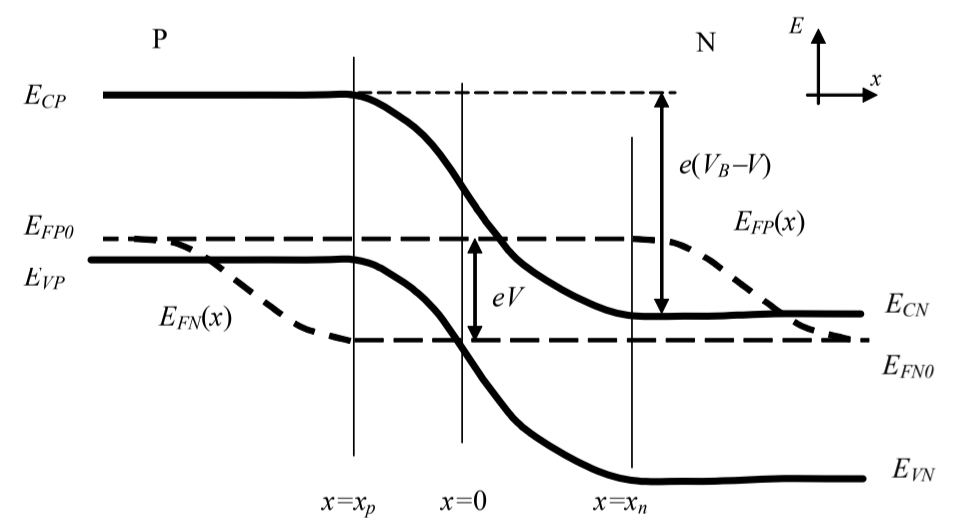
\includegraphics[width=0.60\textwidth]{imagenes/tema4/T4_1_qa.png}
    \caption{Diagrama de cuasiniveles de Fermi en una unión PN bajo polarización inversa.}
    \label{fig:cuasiniveles_inversa}
\end{figure}

\begin{itemize}
    \item \textbf{Lado P:} Los huecos (mayoritarios) apenas sufren variación porcentual en su densidad, por lo que su cuasinivel $E_{FP}$ permanece alineado con el nivel de Fermi del lado P. En cambio, la densidad de electrones (minoritarios) cae fuertemente al aproximarse a la Z.C.E., obligando a su cuasinivel $E_{FN}(x)$ a alejarse del borde de la banda de conducción $E_C(x)$ (hacia abajo).
    \item \textbf{Lado N:} Los electrones (mayoritarios) mantienen su cuasinivel $E_{FN}$ estable, mientras que para los huecos (minoritarios), al disminuir su concentración cerca de $x_n$, su cuasinivel $E_{FP}(x)$ se aleja del borde de la banda de valencia $E_V(x)$ (hacia arriba).
\end{itemize}

\paragraph{2. Polarización directa ($V > 0$)}
Bajo polarización directa, la inyección exponencial de portadores genera un exceso sustancial de concentraciones ($n p > n_i^2$). La separación energética entre los cuasiniveles en la Z.C.E. es exactamente igual al trabajo realizado por la fuente externa: $E_{FN} - E_{FP} = e V$.

\begin{figure}[h!]
    \centering
    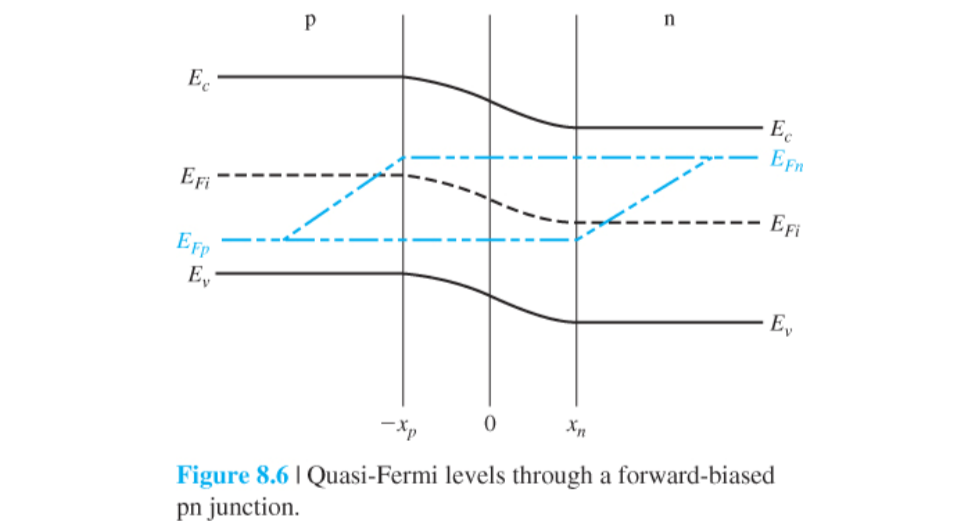
\includegraphics[width=0.60\textwidth]{imagenes/tema4/T4_1_qb.png}
    \caption{Diagrama de cuasiniveles de Fermi en una unión PN bajo polarización directa.}
    \label{fig:cuasiniveles_directa}
\end{figure}

\begin{itemize}
    \item \textbf{Lado P ($x \le -x_p$):} El cuasinivel de mayoritarios $E_{FP}$ permanece constante. Al inyectarse electrones (minoritarios) en la región neutra P, su concentración $n_p(x)$ aumenta significativamente, por lo que el cuasinivel $E_{FN}(x)$ se desplaza hacia arriba, aproximándose al borde de la banda de conducción $E_C(x)$.
    \item \textbf{Lado N ($x \ge x_n$):} El cuasinivel de mayoritarios $E_{FN}$ se mantiene prácticamente inalterado. La inyección de huecos (minoritarios) eleva $p_n(x)$, de modo que el cuasinivel $E_{FP}(x)$ se desplaza hacia abajo, acercándose a la banda de valencia $E_V(x)$.
\end{itemize}

\textbf{Nota:} Aunque en los diagramas esquemáticos los cuasiniveles de Fermi suelen representarse mediante trazos rectlineos ideales en las regiones neutras, en un dispositivo real presentan una curvatura suave asociada al perfil exponencial de recombinación de los portadores minoritarios inyectados.

\newpage

\subsection*{Comportamiento Dinámico}

\subsubsection*{Modelo de Pequeña Señal}

En aplicaciones prácticas de la unión PN, las tensiones y corrientes aplicadas presentan variaciones temporales. Para analizar la respuesta del dispositivo frente a perturbaciones dinámicas de baja amplitud superpuestas a un punto de operación continuo, se utiliza el \textbf{modelo de pequeña señal}.

\paragraph{1. Hipótesis fundamentales del modelo}
\begin{itemize}
    \item \textbf{Aproximación de pequeña señal:} La amplitud de la señal alterna es suficientemente pequeña ($V_i \ll \frac{k_B T}{e} \approx 25,9\,\text{mV}$) como para linealizar la respuesta exponencial del diodo en torno al punto de trabajo.
    \item \textbf{Polarización continua en directa:} La unión permanece en todo momento en la región de polarización directa ($V_0 > 0$).
    \item \textbf{Régimen de baja frecuencia:} La frecuencia $\omega$ de la señal es lo bastante baja como para asumir que el dispositivo atraviesa una sucesión de estados cuasi-estacionarios.
    \item \textbf{Señal excitatriz sinusoidal pura:} La tensión aplicada se expresa en notación fasorial compleja.
\end{itemize}

\begin{figure}[h!]
    \centering
    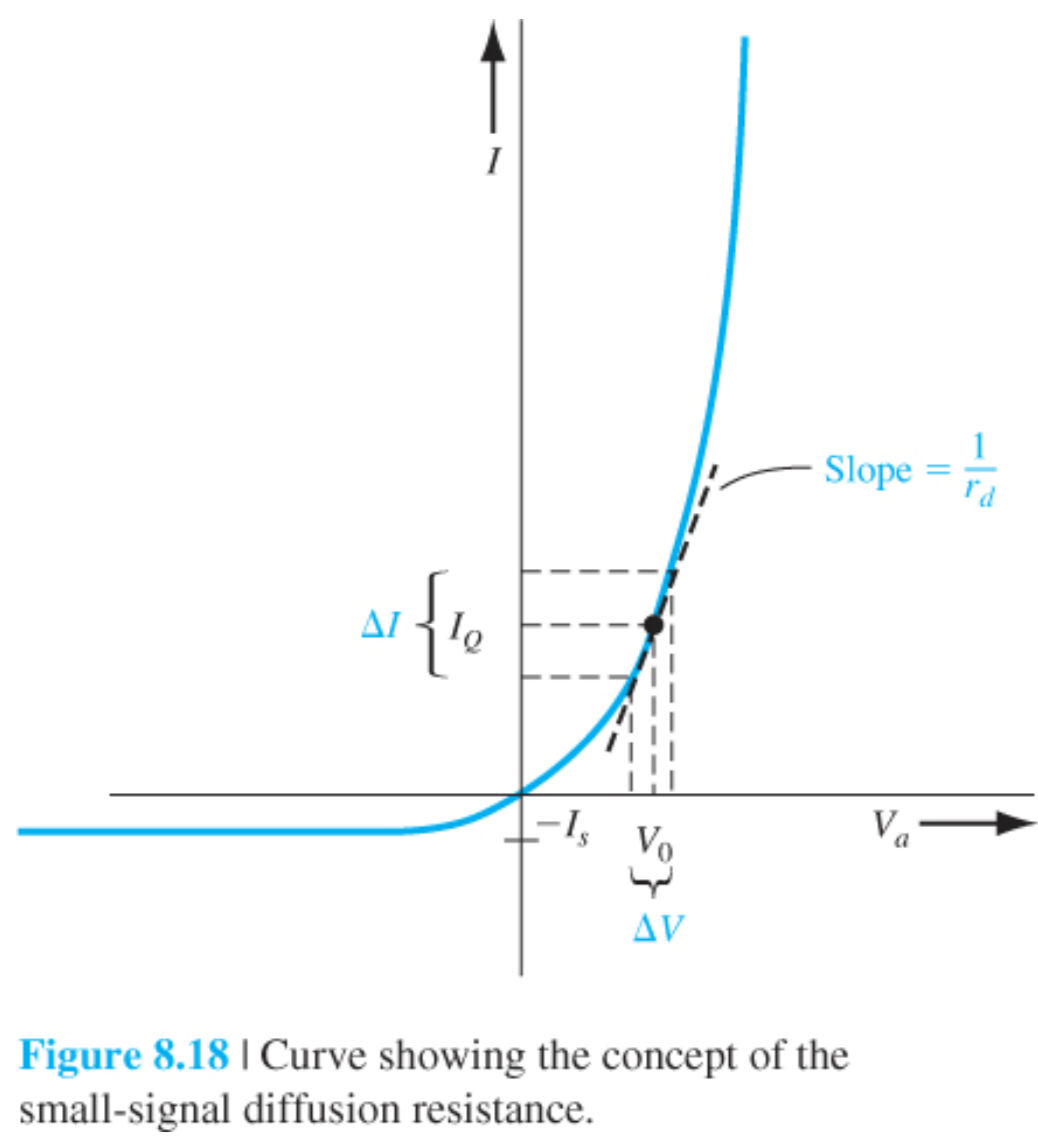
\includegraphics[width=0.65\textwidth]{imagenes/tema4/T4_1_r.png}
    \caption{Unión PN polarizada en directa con una señal alterna de pequeña señal superpuesta a la tensión continua $V_0$ y oscilación de la concentración de portadores minoritarios en el borde de la Z.C.E.}
    \label{fig:pequena_senal_esquema}
\end{figure}

\newpage
\paragraph{2. Tensión aplicada y respuesta en densidad de corriente}
La tensión total aplicada $v(t)$ se compone de un valor continuo $V_0$ y una pequeña variación armónica $v_i(t)$:
\[
v(t) = V_0 + v_i(t) = V_0 + V_i e^{j\omega t}
\]

Debido a la respuesta lineal del sistema para pequeña señal, la densidad de corriente resultante $J(t)$ oscila a la misma frecuencia angular $\omega$:
\[
J(t) = J_0(V_0) + J_1(\omega) e^{j\omega t}
\]
donde $J_0(V_0) = J_0 \left[ \exp\left(\frac{e V_0}{k_B T}\right) - 1 \right]$ es la densidad de corriente continua en el punto de operación estático.

\begin{figure}[h!]
    \centering
    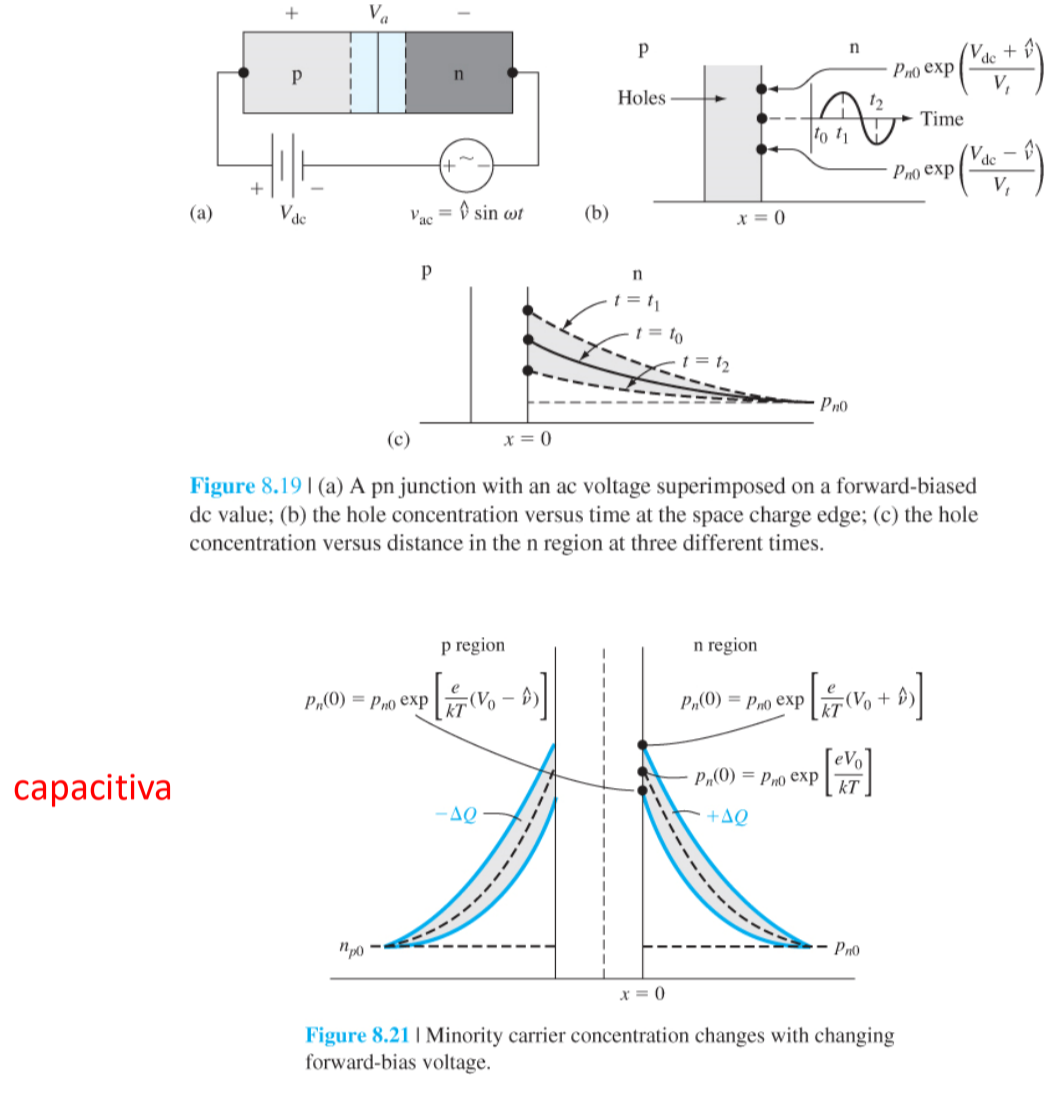
\includegraphics[width=0.75\textwidth]{imagenes/tema4/T4_1_s.png}
    \caption{Concepto de la resistencia de difusión de pequeña señal $r_d = 1/\text{pendiente}$ mediante la linealización de la característica $I-V$ en el punto de operación $(V_0, I_0)$.}
    \label{fig:resistencia_difusion}
\end{figure}

A partir de las componentes alternas se define la \textbf{admitancia compleja de pequeña señal} por unidad de área $Y(\omega)$:
\[
Y(\omega) = \frac{1}{Z(\omega)} = \frac{J_1(\omega)}{V_i(\omega)} = G_d(\omega) + j \omega C_d(\omega)
\]

\newpage
\paragraph{3. Origen físico de las componentes de admitancia}
La respuesta dinámica combina dos mecanismos físicos independientes:
\begin{enumerate}[label=\alph*)]
    \item \textbf{Conductancia de difusión ($G_d = 1/R_d$):} Modela la disipación de potencia asociada a la pendiente de la curva estática $J-V$ en el punto de operación $V_0$.
    \item \textbf{Capacidad de difusión ($C_d$):} Describe el almacenamiento dinámico de carga de portadores minoritarios inyectados en las regiones neutras ($\Delta Q$). Al oscilar la tensión $v_i(t)$, la concentración de portadores minoritarios en las fronteras de la Z.C.E. se modula periódicamente, requiriendo un flujo de carga para ajustar el perfil espacial en cada instante.
\end{enumerate}

\begin{figure}[h!]
    \centering
    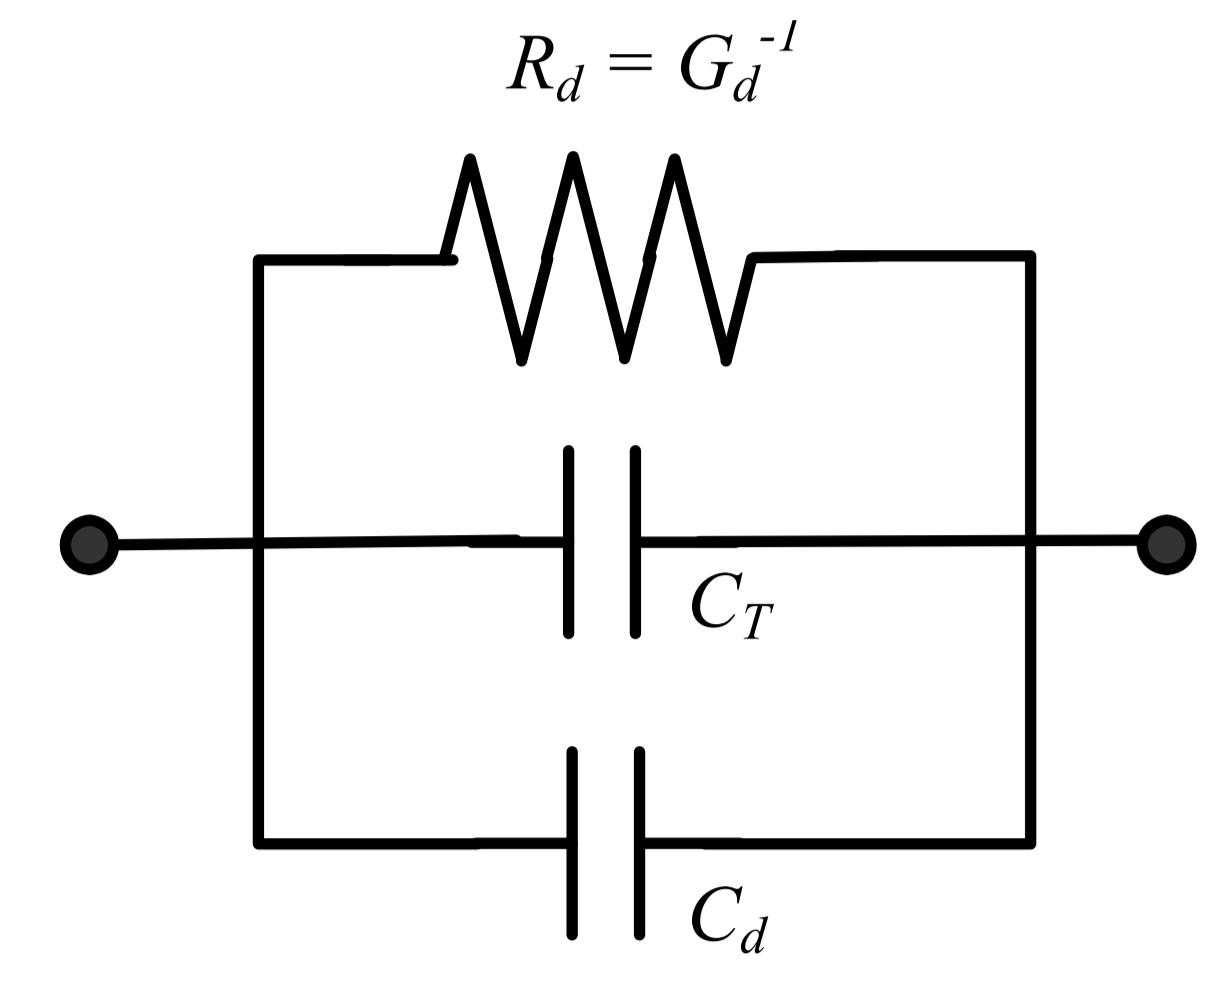
\includegraphics[width=0.65\textwidth]{imagenes/tema4/T4_1_t.png}
    \caption{Variación dinámica del perfil de portadores minoritarios y de la carga almacenada $\pm \Delta Q$ en las regiones neutras bajo régimen de pequeña señal.}
    \label{fig:capacidad_difusion_perfil}
\end{figure}

\newpage
\paragraph{4. Derivación analítica de la admitancia $Y(\omega)$}
Resolviendo la ecuación de continuidad dependiente del tiempo para los portadores minoritarios inyectados en las regiones neutras en régimen fasorial:
\[
j\omega \tilde{p}_n(x) = D_p \frac{d^2 \tilde{p}_n(x)}{dx^2} - \frac{\tilde{p}_n(x)}{\tau_p}
\]

Se obtiene la expresión analítica para la admitancia compleja $Y(\omega)$:
\[
Y(\omega) = \frac{e^2}{k_B T} \left[ \frac{D_p p_{n0}}{L_p} \sqrt{1 + j\omega \tau_p} + \frac{D_n n_{p0}}{L_n} \sqrt{1 + j\omega \tau_n} \right] \exp\left(\frac{e V_0}{k_B T}\right)
\]

Definiendo los factores de conductancia parciales $G_{dp}$ y $G_{dn}$:
\[
G_{dp} = \frac{e^2}{k_B T} \frac{D_p p_{n0}}{L_p} \exp\left(\frac{e V_0}{k_B T}\right), \qquad G_{dn} = \frac{e^2}{k_B T} \frac{D_n n_{p0}}{L_n} \exp\left(\frac{e V_0}{k_B T}\right)
\]
la admitancia se reescribe como:
\[
Y(\omega) = G_{dp} \sqrt{1 + j\omega \tau_p} + G_{dn} \sqrt{1 + j\omega \tau_n}
\]

Separando la parte real e imaginaria para cualquier frecuencia:
\[
\text{Re}[Y(\omega)] = \frac{1}{R_d(\omega, V_0)} = G_{dp} \left[ \frac{1}{2} \sqrt{1 + \omega^2 \tau_p^2} + \frac{1}{2} \right]^{1/2} + G_{dn} \left[ \frac{1}{2} \sqrt{1 + \omega^2 \tau_n^2} + \frac{1}{2} \right]^{1/2}
\]
\[
\text{Im}[Y(\omega)] = \omega C_d(\omega, V_0) = \omega \left\{ \frac{G_{dp}}{\omega} \left[ \frac{1}{2} \sqrt{1 + \omega^2 \tau_p^2} - \frac{1}{2} \right]^{1/2} + \frac{G_{dn}}{\omega} \left[ \frac{1}{2} \sqrt{1 + \omega^2 \tau_n^2} - \frac{1}{2} \right]^{1/2} \right\}
\]

\newpage
\paragraph{5. Aproximación de baja frecuencia ($\omega \tau_p \ll 1, \omega \tau_n \ll 1$)}
En el límite de baja frecuencia, empleamos el desarrollo en serie $\sqrt{1 + j\omega \tau} \approx 1 + \frac{1}{2} j \omega \tau$. La admitancia adopta la forma de un circuito equivalente paralelo $R_d - C_d$ con parámetros independientes de la frecuencia:
\[
Y(\omega) \approx G_d + j \omega C_d
\]

\begin{itemize}
    \item \textbf{Conductancia de difusión en baja frecuencia ($G_d = 1/R_d$):}
    Coincide con la derivada de la densidad de corriente continua en el punto de trabajo $V_0$:
    \[
    G_d = \frac{1}{R_d} = \left. \frac{d J}{d V} \right|_{V=V_0} = \frac{e^2}{k_B T} \left( \frac{D_p p_{n0}}{L_p} + \frac{D_n n_{p0}}{L_n} \right) \exp\left(\frac{e V_0}{k_B T}\right) \approx \frac{e J_0'}{k_B T}
    \]
    donde $J_0' \approx J_0 \exp\left(\frac{e V_0}{k_B T}\right)$ es la densidad de corriente continua en polarización directa.

    \item \textbf{Capacidad de difusión en baja frecuencia ($C_d$):}
    \[
    C_d = \frac{e^2}{2 k_B T} \left( \frac{D_p p_{n0}}{L_p} \tau_p + \frac{D_n n_{p0}}{L_n} \tau_n \right) \exp\left(\frac{e V_0}{k_B T}\right) = \frac{e}{2 k_B T} \left( J_{p0} \tau_p + J_{n0} \tau_n \right) \exp\left(\frac{e V_0}{k_B T}\right)
    \]
    La capacidad de difusión es directamente proporcional a la corriente continua de polarización y a los tiempos de vida media de los portadores minoritarios.
\end{itemize}

\newpage
\paragraph{Análisis en baja frecuencia y naturaleza de la admitancia}
A partir de la solución fasorial de la ecuación de continuidad dependiente del tiempo para portadores minoritarios, la admitancia dinámica por unidad de área adopta la forma general:
\[
Y(\omega) = \frac{1}{R_d(\omega, V_0)} + j \omega C_d(\omega, V_0)
\]

Dado que la parte imaginaria de la admitancia es estrictamente positiva ($\text{Im}[Y] > 0$), la componente reactiva de la respuesta dinámica presenta un \textbf{comportamiento puramente capacitivo}.

Bajo la condición de \textbf{baja frecuencia} ($\omega \tau_n \ll 1$ y $\omega \tau_p \ll 1$), la respuesta del perfil de portadores es capaz de seguir instantáneamente a la señal alterna. Empleando la aproximación de primer orden $\sqrt{1 + j\omega \tau} \approx 1 + j \frac{\omega \tau}{2}$, la admitancia se simplifica a la combinación en paralelo de una conductancia $G_d$ y una capacidad $C_d$, ambas independientes de la frecuencia:
\[
Y = G_d + j \omega C_d
\]

Las expresiones analíticas de ambos parámetros resultan:
\begin{itemize}
    \item \textbf{Conductancia de difusión de pequeña señal ($G_d = 1/R_d$):}
    \[
    G_d = \frac{1}{R_d} = \frac{e^2}{k_B T} \left( \frac{D_p p_{n0}}{L_p} + \frac{D_n n_{p0}}{L_n} \right) \exp\left(\frac{e V_0}{k_B T}\right) = \left. \frac{dJ}{dV} \right|_{V=V_0}
    \]
    Físicamente representa la pendiente de la curva característica estática $J-V$ evaluada en el punto de operación $V_0$.

    \item \textbf{Capacidad de difusión ($C_d$):}
    \[
    C_d = \frac{e^2}{2 k_B T} \left( \frac{D_p p_{n0}}{L_p} \tau_p + \frac{D_n n_{p0}}{L_n} \tau_n \right) \exp\left(\frac{e V_0}{k_B T}\right)
    \]
    Representa la variación de la carga de portadores minoritarios almacenada en las regiones neutras en función de la tensión aplicada.
\end{itemize}

\newpage
\paragraph{Origen de la capacidad de transición y limitación del modelo de continuidad neutra}
Al analizar la expresión de $Y(\omega)$ deducida de la ecuación de continuidad, se observa que únicamente aparece la capacidad de difusión $C_d$. La razón física radica en que dicha deducción se basó exclusivamente en resolver la ecuación de transporte en las \textbf{regiones neutras} fuera de la Z.C.E.

Sin embargo, en la zona de carga espacial existe un almacenamiento estático de carga de iones fijos (aceptores y donadores ionizados) dependiente de la anchura de deplesión $W(V)$. Al variar el voltaje $v(t)$, la anchura $W$ se modula, provocando un flujo de carga de transición a través de las fronteras de la Z.C.E. Esta contribución da lugar a la \textbf{capacidad de transición} (o de deplesión) $C_T$:
\[
C_T = \left( \frac{\epsilon e N_A N_D}{2 (N_A + N_D)} \right)^{1/2} (V_B - V_0)^{-1/2}
\]

\newpage
\subsubsection*{Circuito Equivalente de Pequeña Señal y Baja Frecuencia}

Para modelar de forma completa la respuesta dinámica de la unión PN frente a pequeña señal en baja frecuencia, se conectan en paralelo la resistencia incremental del diodo $R_d = G_d^{-1}$, la capacidad de difusión $C_d$ y la capacidad de transición $C_T$.

\begin{figure}[h!]
    \centering
    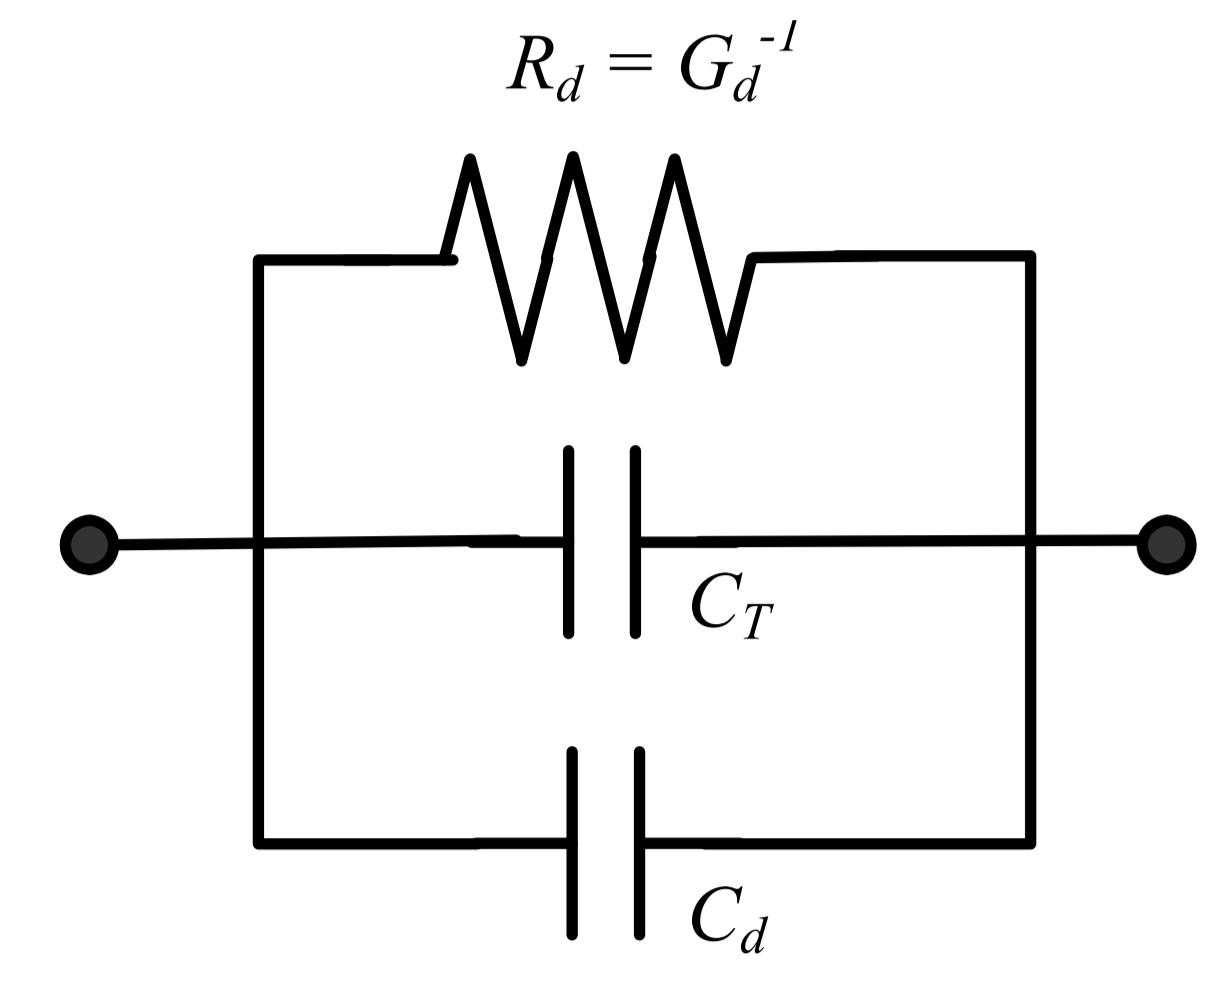
\includegraphics[width=0.45\textwidth]{imagenes/tema4/T4_1_t.png}
    \caption{Circuito equivalente de pequeña señal y baja frecuencia de la unión PN ideal formado por la resistencia incremental $R_d$, la capacidad de transición $C_T$ y la capacidad de difusión $C_d$ en paralelo.}
    \label{fig:circuito_pequena_senal_ideal}
\end{figure}

\paragraph{Predominio de capacidades según el régimen de polarización}
Las dos capacidades asociadas a la unión presentan una dependencia funcional sustancialmente diferente respecto al punto de operación $V_0$:
\begin{itemize}
    \item \textbf{Capacidad de difusión ($C_d$):} Varía de forma \textbf{exponencial} con la tensión aplicada ($\propto \exp(e V_0 / k_B T)$).
    \item \textbf{Capacidad de transición ($C_T$):} Varía de forma \textbf{sublineal} o potencial ($\propto (V_B - V_0)^{-1/2}$).
\end{itemize}

Como consecuencia directa:
\begin{enumerate}[label=\alph*)]
    \item \textbf{En polarización directa ($V_0 > 0$):} La inyección masiva de portadores minoritarios hace que $C_d$ crezca exponencialmente, superando ampliamente a $C_T$ ($C_d \gg C_T$). En este régimen, la capacidad total de la unión es predominantemente la \textbf{capacidad de difusión}.
    \item \textbf{En polarización inversa ($V_0 < 0$):} La concentración de minoritarios se anula en las fronteras, haciendo que $C_d \approx 0$. Aunque $C_T$ disminuye paulatinamente al ensancharse la Z.C.E., pasa a ser la componente claramente dominante ($C_T \gg C_d$).
\end{enumerate}

\newpage
\paragraph{Inclusión de la resistencia serie ($r_s$)}
Para obtener el circuito equivalente real completo del dispositivo, es necesario incorporar el efecto de las pérdidas de conducción en volumen. Cuando el diodo conduce corrientes elevadas en polarización directa, la resistencia incremental $R_d = 1/G_d$ se reduce enormemente. En esta situación, la caída de potencial en las regiones neutras semiconductoras fuera de la Z.C.E. y en las uniones metal-semiconductor de los contactos óhmicos deja de ser despreciable.

Estas pérdidas ohmicas se modelan mediante una \textbf{resistencia serie} $r_s$ conectada en serie con el bloque paralelo de la unión.

\begin{figure}[h!]
    \centering
    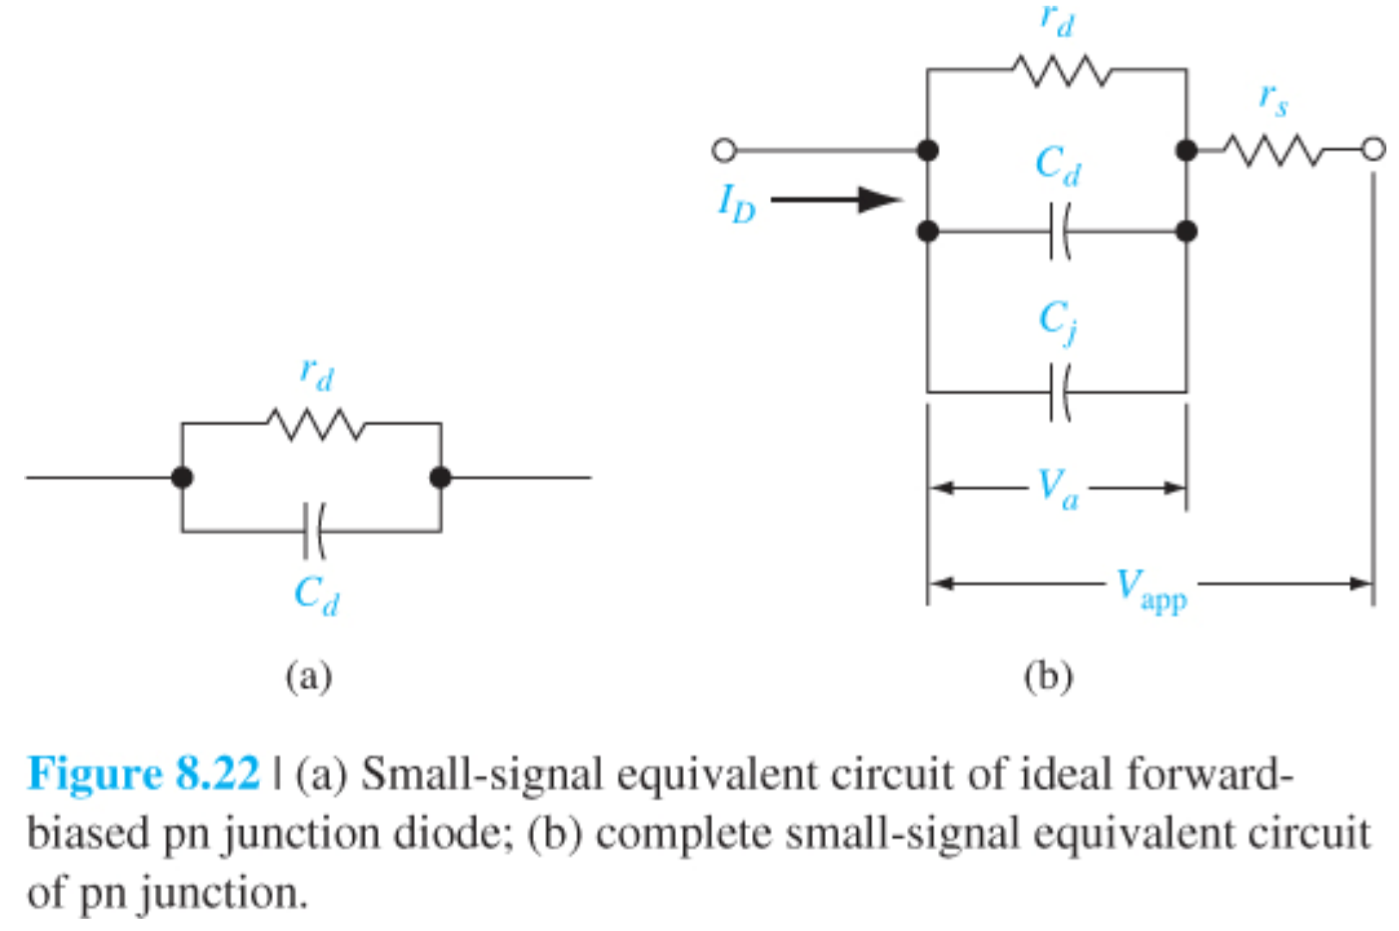
\includegraphics[width=0.75\textwidth]{imagenes/tema4/T4_1_u.png}
    \caption{Circuito equivalente completo de pequeña señal para una unión PN real, incluyendo la resistencia serie $r_s$ de las regiones neutras y contactos óhmicos.}
    \label{fig:circuito_pequena_senal_completo}
\end{figure}

De este modo, la impedancia total de pequeña señal del diodo $Z_{eq}(\omega)$ resulta:
\[
Z_{eq}(\omega) = r_s + \frac{1}{G_d + j \omega (C_d + C_T)} = r_s + \frac{R_d}{1 + j \omega R_d C_j}
\]
donde $C_j = C_d + C_T$ representa la capacidad total equivalente de la unión.

%======================================
% FALTA SECCIÓN!!!!!!!!!!!!!!!!!!!!!!!!!!!!!!!!
%======================================

\newpage
\subsubsection*{Desviaciones del diodo real respecto al ideal}

La ecuación ideal del diodo de Shockley ($J = J_0 [ \exp(e V / k_B T) - 1 ]$) se deriva bajo las hipótesis de ausencia de procesos de generación-recombinación en la Zona de Carga Espacial (Z.C.E.) y débil nivel de inyección en las zonas neutras. Sin embargo, un dispositivo real presenta notables desviaciones experimentales tanto en polarización inversa como en polarización directa.

\begin{figure}[h!]
    \centering
    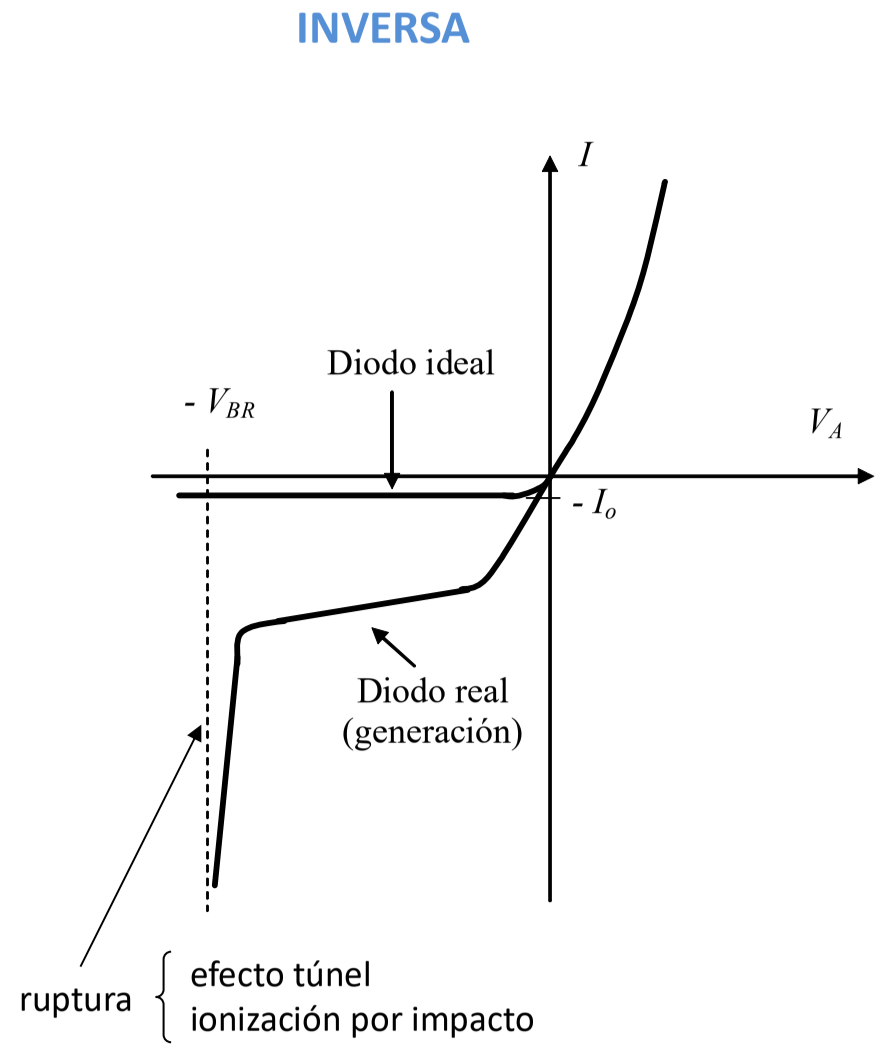
\includegraphics[width=0.60\textwidth]{imagenes/tema4/T4_1_v.png}
    \caption{Curva característica $I-V$ comparativa entre el diodo ideal y el diodo real bajo polarización inversa y región de ruptura.}
    \label{fig:diodo_real_inversa}
\end{figure}

\paragraph{1. Comportamiento en polarización inversa ($V < 0$)}
En un diodo ideal, la corriente en inversa se satura a un valor constante $I = -I_0$. En un dispositivo real, la magnitud de la corriente inversa supera a $I_0$ y crece paulatinamente con la tensión aplicada debido a dos fenómenos físicos principales:

\begin{enumerate}[label=\alph*)]
    \item \textbf{Corriente de generación en la Z.C.E. ($J_{\text{gen}}$):}
    Bajo polarización inversa, la deplesión de portadores en la Z.C.E. origina una condición de defecto estricto ($n p \ll n_i^2$). Para restablecer el equilibrio térmico, los centros de recombinación en la Z.C.E. actúan como centros de generación neta (mecanismo Shockley-Read-Hall). 

    Cada par electrón-hueco generado térmicamente en la Z.C.E. es separado inmediatamente por el campo eléctrico intenso: el hueco es arrastrado hacia la región P y el electrón hacia la región N. Esta contribución da lugar a la corriente de generación $J_{\text{gen}}$, la cual es proporcional al volumen de la Z.C.E. y, por ende, a la anchura $W(V) \propto \sqrt{V_B + |V|}$:
    \[
    J_{\text{rev, real}} = -(J_0 + J_{\text{gen}}), \qquad J_{\text{gen}} \approx \frac{e n_i W(V)}{2 \tau_0}
    \]

    \begin{figure}[h!]
        \centering
        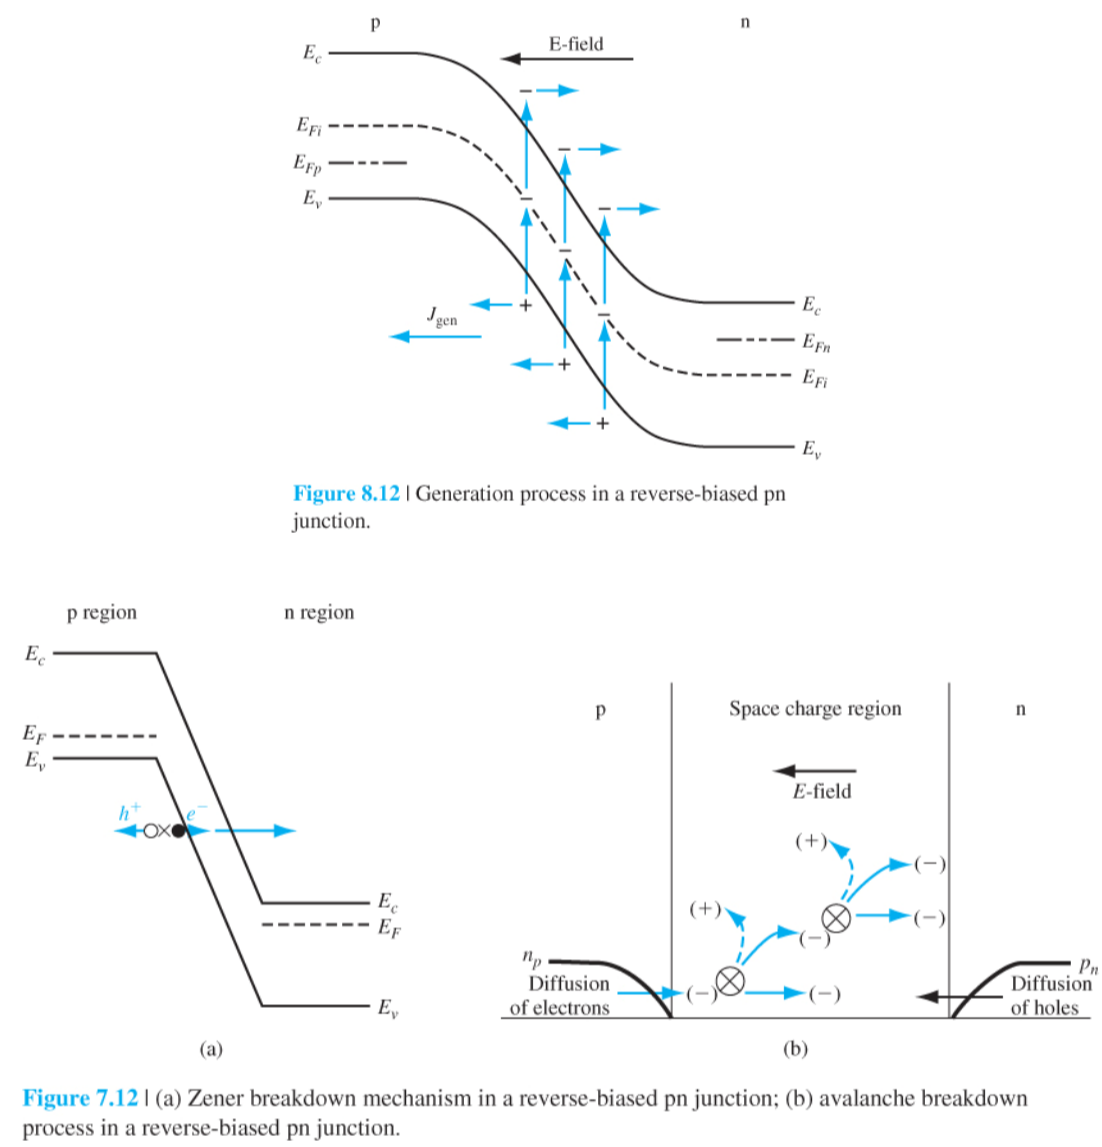
\includegraphics[width=0.75\textwidth]{imagenes/tema4/T4_1_w.png}
        \caption{Mecanismo de generación de pares electrón-hueco en la zona de carga espacial bajo polarización inversa.}
        \label{fig:mecanismo_generacion_zce}
    \end{figure}

    \item \textbf{Fenómenos de ruptura en inversa ($V = -V_{BR}$):}
    Al alcanzar una tensión inversa crítica denominada \textbf{voltaje de ruptura} ($V_{BR}$), la corriente en inversa aumenta drásticamente sin que se incremente apreciablemente la caída de tensión. Este comportamiento viene provocado por dos mecanismos microscópicos:
    \begin{itemize}
        \item \textbf{Ionización por impacto (Ruptura por avalancha):}
        Ocurre en uniones con niveles de dopado moderados o bajos, donde la Z.C.E. es ancha. El elevado campo eléctrico acelera a los portadores minoritarios incidentes hasta alcanzar una energía cinética suficiente como para colisionar con un electrón de valencia de la red y promoverlo a la banda de conducción, creando un nuevo par electrón-hueco. Los nuevos portadores generados se aceleran a su vez, multiplicando de forma en cascada o "en avalancha" la densidad de corriente.
        \item \textbf{Efecto Túnel (Ruptura Zener):}
        Predomina en uniones muy fuertemente dopadas ($P^+ N^+$ o uniones degeneradas). La elevada concentración de impurezas reduce la anchura $W$ de la Z.C.E. a unos pocos nanómetros, haciendo que el gradiente de energía entre la banda de valencia del lado P y la banda de conducción del lado N sea sumamente estrecho. Bajo estas condiciones, los electrones de valencia del lado P pueden atravesar la barrera de potencial por efecto túnel cuántico directo hacia los estados vacíos de la banda de conducción del lado N.
    \end{itemize}
\end{enumerate}

\newpage
\paragraph{2. Comportamiento en polarización directa ($V > 0$)}
En polarización directa, la característica experimental $\ln(I) - V$ muestra tres regiones diferenciadas asociadas a distintas desviaciones respecto al modelo ideal:

\begin{figure}[h!]
    \centering
    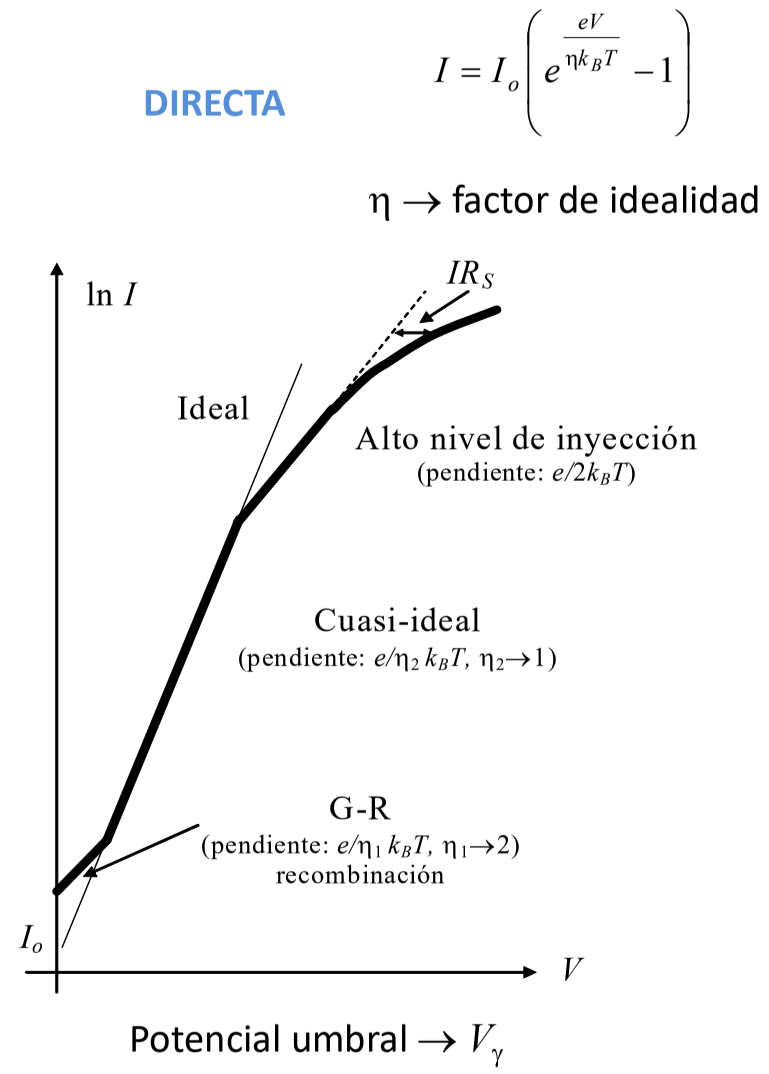
\includegraphics[width=0.60\textwidth]{imagenes/tema4/T4_1_x.png}
    \caption{Curva característica $\ln(I)$ en función de la tensión en directa $V$, ilustrando las regiones de recombinación en la Z.C.E., comportamiento cuasi-ideal y alto nivel de inyección/resistencia serie.}
    \label{fig:diodo_real_directa_ln}
\end{figure}

\begin{enumerate}[label=\alph*)]
    \item \textbf{Región de baja tensión (Dominio de la recombinación en la Z.C.E.):}
    A valores pequeños de tensión en directa, la inyección de portadores desde los bordes genera un exceso en la Z.C.E. ($n p > n_i^2$). Una parte considerable de los portadores inyectados se recombina en el interior de la propia Z.C.E. antes de alcanzar las regiones neutras, originando una componente de corriente de recombinación $J_{\text{rec}} \propto \exp(e V / 2 k_B T)$. Esta corriente adicional supera a la corriente de difusión ideal, produciendo una desviación observada como una mayor corriente experimental en directa respecto a la teórica.

    \item \textbf{Región de tensión moderada (Régimen cuasi-ideal):}
    A medida que la tensión aumenta, la corriente de difusión de minoritarios en las regiones neutras pasa a ser el mecanismo dominante frente a la recombinación en la Z.C.E. El diodo sigue fielmente el comportamiento exponencial teórico.

    \item \textbf{Región de elevada tensión (Alto nivel de inyección y caída óhmica serie):}
    A corrientes elevadas, la concentración de portadores minoritarios inyectados alcanza un orden de magnitud comparable a la densidad de portadores mayoritarios en equilibrio ($p_n \approx N_d$ o $n_p \approx N_a$), entrando en el régimen de \textbf{alto nivel de inyección}. La pendiente de la curva logarítmica se reduce a la mitad ($e / 2 k_B T$). 

    Asimismo, la caída de tensión óhmica en la resistencia serie de las regiones neutras y contactos ($I r_s$) pasa a ser apreciable. La tensión efectiva sobre la unión decrece a $V_j = V_{\text{aplicado}} - I r_s$, provocando que la característica $I-V$ doble suavemente hacia una recta con comportamiento marcadamente resistivo.
\end{enumerate}

\newpage
\paragraph{3. Factor de idealidad ($\eta$) y Potencial Umbral ($V_\gamma$)}
Para englobar cuantitativamente estas desviaciones físicas en la ecuación analítica del diodo, se introduce el \textbf{factor de idealidad} $\eta$:
\[
I = I_0 \left[ \exp\left(\frac{e V}{\eta k_B T}\right) - 1 \right]
\]

El valor numérico de $\eta$ varía dinámicamente según el régimen de operación predominante:
\begin{itemize}
    \item $\eta \approx 2$ a bajas tensiones en directa (dominado por la recombinación en la Z.C.E.).
    \item $\eta \rightarrow 1$ a tensiones moderadas (comportamiento cuasi-ideal gobernado por difusión).
    \item $\eta \approx 2$ a muy altas tensiones (alto nivel de inyección).
\end{itemize}

\begin{figure}[h!]
    \centering
    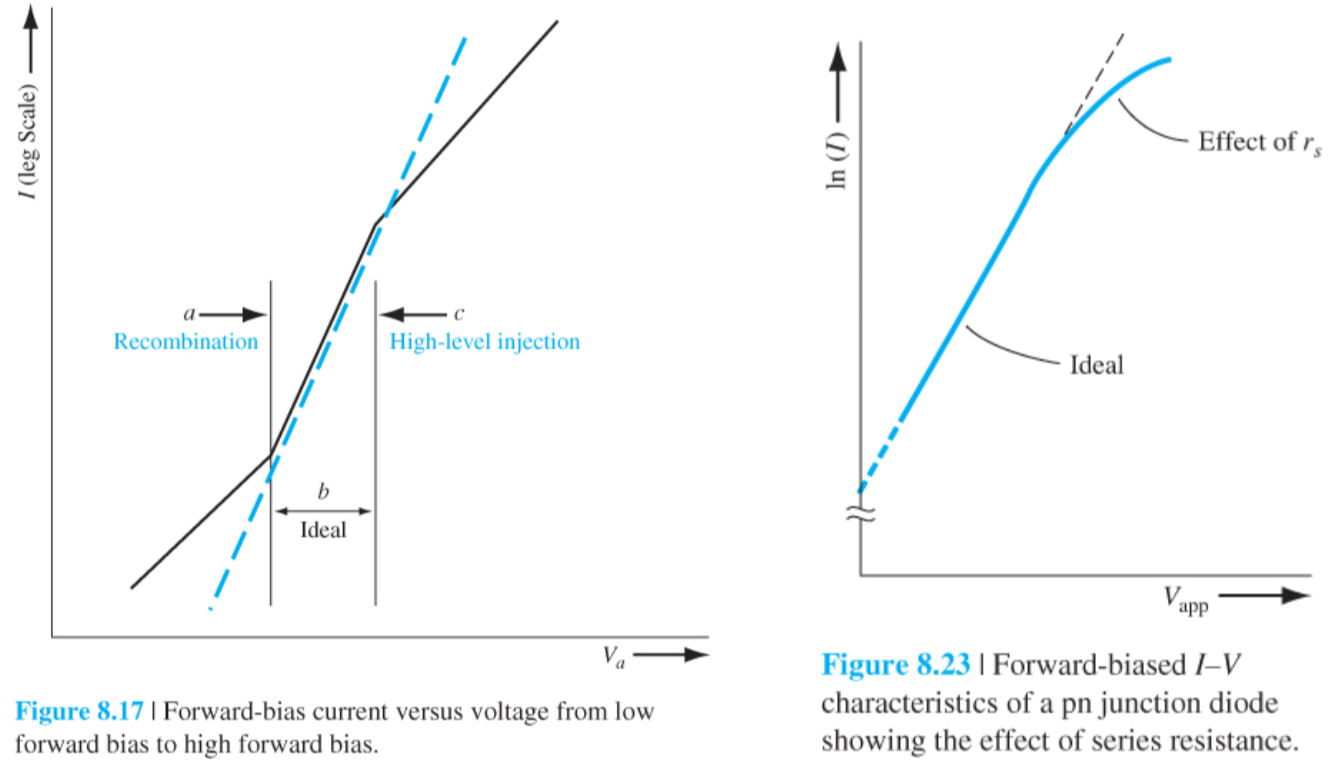
\includegraphics[width=0.75\textwidth]{imagenes/tema4/T4_1_y.png}
    \caption{Definición del potencial umbral o tensión de codo $V_\gamma$ en la característica lineal $I-V$ de un diodo real.}
    \label{fig:potencial_umbral}
\end{figure}

Finalmente, se define el \textbf{potencial umbral} (o tensión de codo $V_\gamma$) como el valor explícito de tensión en directa a partir del cual la corriente del diodo empieza a crecer de forma apreciable en escala lineal (típicamente $V_\gamma \approx 0,6 - 0,7\,\text{V}$ para el silicio y $V_\gamma \approx 0,2 - 0,3\,\text{V}$ para el germanio).









\newpage
%===============================================
%====== SECCIÓN. PROBLEMAS RESUELTOS ===========
%===============================================
\seccionproblemas
%===================
% Problema 01: Unión P-N+ polarizada (Diodo corto)
%===================
\begin{problema}[Unión $P-N^+$ en régimen de polarización y diodo corto]
Para el silicio a $T = \SI{300}{\kelvin}$ ($k_B T = \SI{0.026}{\eV}$), se consideran los siguientes parámetros:
\[
N_c = \SI{2.83e19}{\cm^{-3}}, \quad N_v = \SI{1.10e19}{\cm^{-3}}, \quad n_i = \SI{6.9e9}{\cm^{-3}}, \quad E_g = \SI{1.12}{\eV}
\]
\[
\mu_n = \SI{1500}{\cm^2/\V\second}, \quad \mu_p = \SI{450}{\cm^2/\V\second}, \quad \epsilon = \SI{1.05e-12}{\farad\per\cm}
\]
siendo las longitudes de difusión de los portadores $L_n = \SI{60}{\um}$ y $L_p = \SI{50}{\um}$.

Se realiza una unión $P-N^+$ con este semiconductor, estando el lado $P$ compuesto por una región de longitud $W_P = \SI{5}{\um}$ acabada en un contacto óhmico e impurificada uniformemente con $N_A^- = \SI{1.5e14}{\cm^{-3}}$. El semiconductor tipo $N^+$ está muy impurificado, de tal forma que su nivel de Fermi coincide con el fondo de la banda de conducción ($E_{Fn} = E_C$).

\begin{enumerate}[label=\alph*)]
    \item Calcular la polarización $V$ que se debe aplicar a la unión para que la anchura de su zona de carga espacial sea de $\SI{1.5}{\um}$.
    \item ¿Qué corriente circulará por la unión en esta situación de polarización?
\end{enumerate}
\tcblower
\textbf{Consideración previa: Modelo de diodo corto}

La longitud física total del semiconductor tipo $P$ es $W_P = \SI{5}{\um}$. Al formarse la zona de carga espacial con una anchura $|x_p| = \SI{1.5}{\um}$, la longitud efectiva de la zona neutra resulta:
\[
W_P' = W_P - |x_p| = \SI{5}{\um} - \SI{1.5}{\um} = \SI{3.5}{\um}
\]

Dado que $W_P' = \SI{3.5}{\um} \ll L_n = \SI{60}{\um}$, nos encontramos ante un \textbf{diodo corto}. Por tanto, se puede despreciar la generación y recombinación en el volumen de la zona neutra del lado $P$.

\paragraph{a) Cálculo de la polarización aplicada $V$}

Por tratarse de una unión asimétrica $P-N^+$ ($N_D \gg N_A$), la zona de carga espacial se extiende casi en su totalidad hacia el lado menos dopado ($P$), de modo que $x_n \approx 0$ y $W \approx |x_p|$. 

La anchura de la zona de carga espacial en el lado $P$ bajo una tensión aplicadas $V$ viene dada por:
\[
|x_p| = \sqrt{\frac{2\epsilon (V_B - V)}{e N_A}} \implies V = V_B - \frac{e N_A |x_p|^2}{2\epsilon}
\]

Para determinar el potencial de contacto $V_B$, calculamos la posición del nivel de Fermi en la región $P$ respecto de la banda de valencia:
\[
p_{p0} = N_A = N_v \exp\left(-\frac{E_{Fp} - E_V}{k_B T}\right) \implies E_{Fp} - E_V = k_B T \ln\left(\frac{N_v}{N_A}\right)
\]
\[
E_{Fp} - E_V = (\SI{0.026}{\eV}) \ln\left(\frac{\num{1.10e19}}{\num{1.5e14}}\right) \approx \SI{0.291}{\eV}
\]

Puesto que en el semiconductor $N^+$ el nivel de Fermi coincide con el fondo de la banda de conducción ($E_{Fn} = E_C$), la barrera de potencial interna $V_B$ es:
\[
e V_B = E_{Fn} - E_{Fp} = E_C - E_{Fp} = E_g - (E_{Fp} - E_V) = \SI{1.12}{\eV} - \SI{0.291}{\eV} = \SI{0.829}{\eV}
\]
\[
V_B = \SI{0.829}{\V}
\]

\begin{center}
    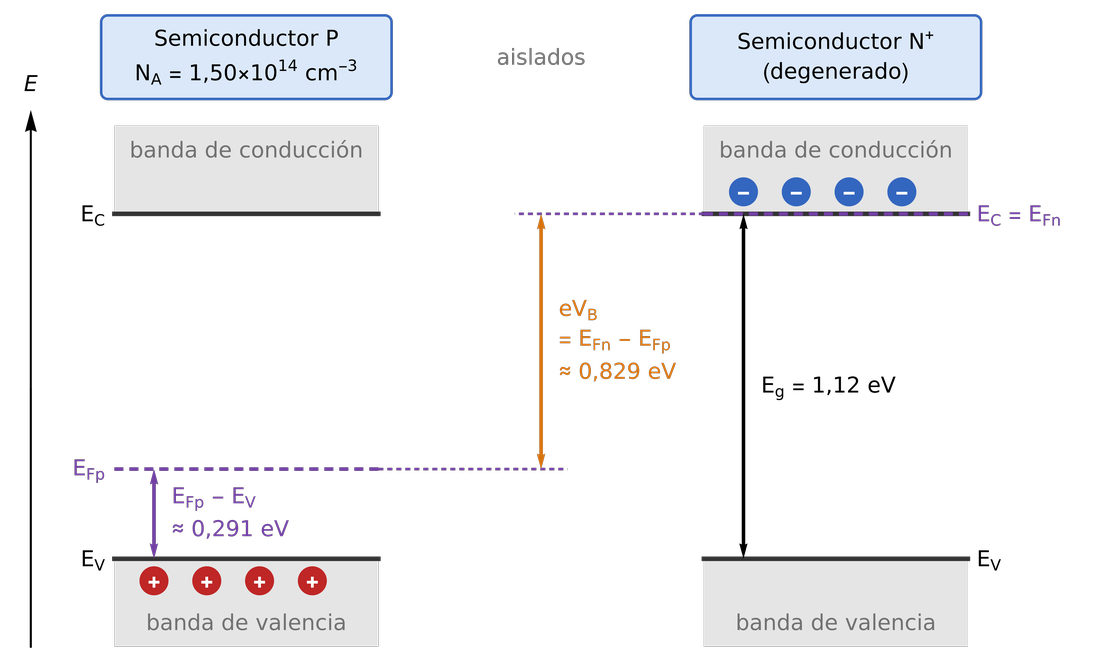
\includegraphics[width=0.55\textwidth]{imagenes/tema4/T4_P1_a.png}
    \captionof{figure}{Diagrama de bandas de energía de los semiconductores P y N+ aislados para ilustrar el potencial de contacto $V_B$.}
\end{center}

A modo de comprobación, la anchura de deplesión en equilibrio ($V = 0$) sería:
\[
|x_p|_{V=0} = \sqrt{\frac{2 \epsilon V_B}{e N_A}} = \sqrt{\frac{2 \times (\num{1.05e-12}) \times 0.829}{(\num{1.6e-19}) \times (\num{1.5e14})}} = \SI{2.69e-4}{\cm} = \SI{2.69}{\um}
\]

Para reducir la zona de carga espacial a $|x_p| = \SI{1.5}{\um} = \SI{1.5e-4}{\cm}$, la polarización en directa $V$ necesaria es:

\begin{align*}
    V & = \SI{0.829}{\V} - \frac{(\num{1.6e-19}\,\text{C}) \times (\num{1.5e14}\,\text{cm}^{-3}) \times (\num{1.5e-4}\,\text{cm})^2}{2 \times (\num{1.05e-12}\,\text{F/cm})} = \\
    & = 0.829 - 0.257 = \SI{0.572}{\V} \approx \SI{0.57}{\V}
\end{align*}

\paragraph{b) Cálculo de la densidad de corriente $J$}

En una unión $P-N^+$, la corriente total está dominada ampliamente por la inyección de electrones minoritarios en el lado $P$ ($J \approx J_n$).

La ecuación de continuidad estacionaria sin recombinación en la zona neutra se reduce a:
\[
\frac{d^2 n_p}{dx^2} = 0 \implies n_p(x) \text{ presenta una variación lineal}
\]

Estableciendo las condiciones de contorno en las fronteras de la región neutra $P$ (entre $x_L = -\SI{5}{\um}$ y $x_p = -\SI{1.5}{\um}$):
\begin{enumerate}
    \item En la frontera de la Z.C.E. ($x = x_p$): $n_p(x_p) = n_{p0} \exp\left(\frac{e V}{k_B T}\right)$.
    \item En el contacto óhmico ideal ($x = x_L$): $n_p(x_L) = n_{p0}$.
\end{enumerate}

La pendiente del perfil de concentración es constante:
\[
\frac{dn_p}{dx} = \frac{n_p(x_p) - n_p(x_L)}{x_p - x_L} = \frac{n_{p0} \left[ \exp\left(\frac{e V}{k_B T}\right) - 1 \right]}{W_P'}
\]

Obtenemos los parámetros numéricos involucrados:
\begin{itemize}
    \item Coeficiente de difusión de electrones: $D_n = \frac{k_B T}{e} \mu_n = (\SI{0.026}{\V}) \times (\SI{1500}{\cm^2/\V\second}) = \SI{39}{\cm^2/\second}$.
    \item Densidad de electrones minoritarios en equilibrio: $n_{p0} = \frac{n_i^2}{N_A} = \frac{(\num{6.9e9})^2}{\num{1.5e14}} = \SI{3.174e5}{\cm^{-3}}$.
    \item Longitud de la región neutra: $W_P' = \SI{3.5}{\um} = \SI{3.5e-4}{\cm}$.
\end{itemize}

Evaluando la densidad de corriente de difusión de electrones:
\[
J \approx J_n = e D_n \frac{dn_p}{dx} = \frac{e D_n n_{p0}}{W_P'} \left[ \exp\left(\frac{e V}{k_B T}\right) - 1 \right]
\]

Sustituyendo los valores para $V = \SI{0.57}{\V}$:
\begin{align*}
    J & = \frac{(\num{1.6e-19}) \times 39 \times (\num{3.174e5})}{\num{3.5e-4}} \left[ \exp\left(\frac{0.57}{0.026}\right) - 1 \right] \\
    & = (\num{5.65e-10}) \times (\num{3.319e9}) \approx \SI{18.76}{\A\per\cm^2}
\end{align*}

\textit{Nota:} Si se toma el valor exacto de la tensión $V = \SI{0.5716}{\V}$, la densidad de corriente resulta $J \approx \SI{19.96}{\A\per\cm^2}$.
\end{problema}
\newpage
%===================
% Problema 02: Diodo corto P+-N
%===================
\begin{problema}[Diodo corto $P^+-N$ y perforación de la zona neutra]
Sobre un bloque de silicio tipo N no degenerado, cúbico de arista $L = \SI{10}{\um}$, se construye un diodo corto ($L_p \gg \SI{10}{\um}$) depositando sobre una cara un contacto óhmico (el cual se comporta como un sumidero perfecto del exceso de portadores) y sobre la cara opuesta silicio tipo $P^+$ (degenerado, de forma tal que $E_{Fp} = E_V$). De esta estructura además se sabe que a $T = \SI{300}{\kelvin}$ la resistencia de la zona tipo N entre las caras paralelas es $R = \SI{10.38}{\kilo\ohm}$.

Calcular:
\begin{enumerate}[label=\alph*)]
    \item Potencial de contacto $V_B$ de la unión $P^+-N$ así formada.
    \item Anchura de la zona de transición y capacidad de transición de la unión en función del potencial aplicado $V$.
    \item Distribución de portadores en la zona N, evaluando la influencia que en ella pueda tener el potencial aplicado.
    \item Característica $I-V$ de la unión. Coméntese el comportamiento en polarización inversa.
\end{enumerate}

\textbf{Datos del semiconductor a $T = \SI{300}{\kelvin}$ ($k_B T = \SI{0.026}{\eV}$):}
\[
n_i = \SI{6.9e9}{\cm^{-3}}, \quad N_c = \SI{2.83e19}{\cm^{-3}}, \quad N_v = \SI{1.10e19}{\cm^{-3}}, \quad E_g = \SI{1.12}{\eV}
\]
\[
\mu_n = \SI{1500}{\cm^2/\V\second}, \quad \mu_p = \SI{450}{\cm^2/\V\second}, \quad \epsilon = \SI{1.061e-12}{\farad\per\cm}
\]
\tcblower
\textbf{a) Potencial de contacto de la unión $P^+-N$}

La resistencia de la región semiconductora tipo N de sección transversal $A = L^2$ y longitud $L = \SI{10}{\um} = \SI{10e-4}{\cm}$ se expresa como:
\[
R = \frac{L}{\sigma A} = \frac{L}{e \mu_n n_{n0} L^2} = \frac{1}{e \mu_n n_{n0} L}
\]

Despejando la concentración de electrones mayoritarios en equilibrio $n_{n0} \approx N_D$:
\[
\begin{aligned}
N_D = n_{n0} &= \frac{1}{e\,\mu_n\,R\,L} \\
&= \frac{1}{(\SI{1.6e-19}{\coulomb})\,(\SI{1500}{\cm\squared\per\volt\per\second})\,(\SI{10.38e3}{\ohm})\,(\SI{10e-4}{\cm})} \\
&= \SI{4.014e14}{\per\cm\cubed}
\end{aligned}
\]

La separación del nivel de Fermi en el lado N respecto al fondo de la banda de conducción $E_C$ es:
\[
E_C - E_{Fn} = k_B T \ln\left(\frac{N_c}{n_{n0}}\right) = (\SI{0.026}{\eV}) \ln\left(\frac{\num{2.83e19}}{\num{4.014e14}}\right) \approx \SI{0.291}{\eV} \quad (\approx \SI{0.28}{\eV})
\]

Puesto que el lado $P^+$ está fuertemente degenerado ($E_{Fp} = E_V$), la barrera de potencial interno $V_B$ resulta:
\[
e V_B = E_{Fn} - E_{Fp} = E_C - (E_C - E_{Fn}) - E_V = E_g - (E_C - E_{Fn}) = \SI{1.12}{\eV} - \SI{0.28}{\eV} = \SI{0.84}{\eV}
\]
\[
V_B = \SI{0.84}{\V} \quad (\text{o bien } \SI{0.83}{\V} \text{ tomando el valor no redondeado})
\]

\textbf{b) Anchura y capacidad de la zona de transición en función de $V$}

Por tratarse de una unión asimétrica $P^+-N$ ($N_A \gg N_D$), la zona de carga espacial penetra de forma casi exclusiva en el lado menos dopado N ($x_p \approx 0$), resultando $W(V) \approx x_n(V)$:
\[
x_n(V) = \sqrt{\frac{2\epsilon (V_B - V)}{e N_D}} = \sqrt{\frac{2 \times (\num{1.061e-12})}{\num{1.6e-19} \times \num{4.014e14}}} \sqrt{0.84 - V} = \SI{1.82e-4}{\cm} \sqrt{0.84 - V}
\]
\[
x_n(V) = 1.82 \sqrt{0.84 - V} \quad (\si{\um}, \text{con } V \text{ en voltios})
\]

La capacidad de transición $C(V)$ para la superficie $A = L^2 = (\SI{10e-4}{\cm})^2 = \SI{1e-6}{\cm\squared}$ es:
\[
\begin{aligned}
C(V) &= \frac{\epsilon A}{x_n(V)}
= \frac{(\SI{1.061e-12}{\farad\per\cm})\,(\SI{1e-6}{\cm\squared})}{\SI{1.82e-4}{\cm}}\,(0.84 - V)^{-1/2} \\
&= \num{5.83e-15}\,(0.84 - V)^{-1/2} \quad (\si{\farad})
\end{aligned}
\]

\textbf{c) Distribución de portadores en la zona N}

Al ser un diodo corto ($L - x_n \ll L_p$), se desprecia la recombinación en el volumen de la región neutra N ($x_n \le x \le L$). La ecuación de continuidad estacionaria simplificada se reduce a:
\[
\frac{d^2 p_n}{dx^2} = 0 \implies p_n(x) \text{ es una distribución lineal}
\]

Imponiendo las condiciones de contorno:
\begin{enumerate}
    \item En la frontera de la Z.C.E. ($x = x_n$): $p_n(x_n) = p_{n0} \exp\left(\frac{e V}{k_B T}\right)$.
    \item En el contacto óhmico ideal ($x = L$): $p_n(L) = p_{n0}$ (sumidero perfecto de portadores).
\end{enumerate}

La recta que satisface ambas condiciones es:
\[
p_n(x) = p_{n0} + \frac{p_{n0}\left[\exp\left(\frac{e V}{k_B T}\right) - 1\right]}{x_n - L} (x - L) = p_{n0} + \frac{p_{n0}\left[\exp\left(\frac{e V}{k_B T}\right) - 1\right]}{L - x_n(V)} (L - x)
\]

Bajo polarización directa ($V > 0$), se establece un perfil decreciente positivo inyectado hacia el contacto óhmico. Bajo polarización inversa ($V < 0$), el perfil presenta pendiente positiva con deplesión en la frontera $x = x_n$.

\textbf{d) Característica $I-V$ y comentario sobre la polarización inversa}

Al ser una unión $P^+-N$, la corriente está dominada totalmente por la difusión de huecos minoritarios en el lado N:
\[
J \approx J_p(x_n) = -e D_p \left. \frac{dp_n}{dx} \right|_{x_n} = \frac{e D_p p_{n0}}{L - x_n(V)} \left[ \exp\left(\frac{e V}{k_B T}\right) - 1 \right]
\]

Con $D_p = \frac{k_B T}{e} \mu_p = (\SI{0.026}{\V}) \times (\SI{450}{\cm^2/\V\second}) = \SI{11.7}{\cm^2/\second}$ y $p_{n0} = \frac{n_i^2}{N_D} = \frac{(\num{6.9e9})^2}{\num{4.014e14}} = \SI{1.186e5}{\cm^{-3}}$, la corriente total $I(V) = J(V) \cdot A$ es:
\[
I(V) = \frac{e D_p p_{n0} L^2}{L - x_n(V)} \left[ \exp\left(\frac{e V}{k_B T}\right) - 1 \right]
\]

\textbf{Comentario sobre la polarización inversa y efecto de perforación (Punch-through):}
\begin{itemize}
    \item En un diodo largo, la corriente en inversa se satura a un valor constante. En cambio, en este diodo corto, para $V < 0$ se tiene $\exp(e V / k_B T) \approx 0$ y la corriente inversa resulta:
    \[
    I_{\text{rev}} \approx -\frac{e D_p p_{n0} L^2}{L - x_n(V)}
    \]
    Puesto que la anchura de deplesión $x_n(V)$ aumenta con el voltaje inverso $|V|$, la longitud de la zona neutra $W_N' = L - x_n(V)$ se reduce progresivamente, aumentando el gradiente de concentración de huecos. Por tanto, \textbf{la corriente inversa en un diodo corto no es constante, sino que aumenta en módulo al elevar la tensión inversa}.
    
    \item \textbf{Perforación (Punch-through):} Si la tensión inversa se incrementa hasta que la zona de carga espacial alcanza el contacto óhmico opuesto ($x_n = L = \SI{10}{\um} = \SI{10e-4}{\cm}$):
    \[
    1.82 \times 10^{-4} \sqrt{0.84 - V_{PT}} = 10 \times 10^{-4} \implies 0.84 - V_{PT} \approx 30.2 \implies V_{PT} \approx \SI{-29.4}{\V}
    \]
    A esta tensión de perforación ($V_{PT} \approx \SI{-29.4}{\V}$), la zona neutra desaparece ($W_N' \to 0$), destruyendo la barrera de potencial y provocando un incremento masivo de corriente que destruye térmicamente la unión.
\end{itemize}

\begin{center}
    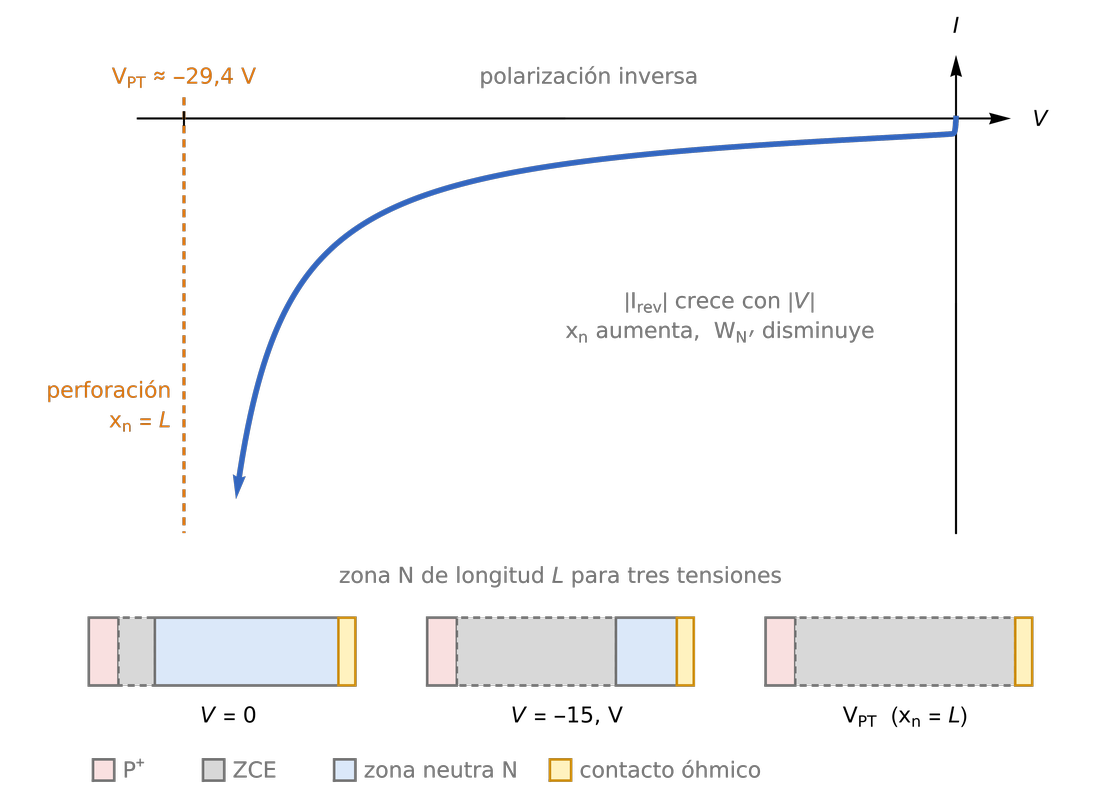
\includegraphics[width=0.55\textwidth]{imagenes/tema4/T4_P2_b.png}
    \captionof{figure}{Característica $I-V$ en polarización inversa para un diodo corto, mostrando el aumento de la corriente con la tensión y el fenómeno de perforación (punch-through).}
\end{center}
\end{problema}